% Fix hyperref/kernel mismatch (TeX Live 2025): define \IfDocumentMetadataT so pdflatex exits 0 and latexmk runs twice to generate TOC
\makeatletter
\providecommand{\IfDocumentMetadataT}[1]{#1}
\makeatother

\documentclass{mcmthesis}
\mcmsetup{tstyle=\color{red}\bfseries,
        tcn = 2631703, problem = C,
        sheet = true, titleinsheet = true, keywordsinsheet = true,
        titlepage = false, abstract = true}

\usepackage{times}
\usepackage{indentfirst}
\usepackage{lipsum}
\usepackage{amsmath}
\usepackage{amssymb}
\usepackage{graphicx}
\usepackage{booktabs}
\usepackage{longtable}
\usepackage{arydshln}
\usepackage{multirow}
\usepackage{hyperref}
\usepackage{tocloft}
\usepackage{float}
\renewcommand{\contentsname}{\textbf{Contents}}
\setlength{\cftbeforesecskip}{0.5em}
\setlength{\cftbeforesubsecskip}{0.25em}
\renewcommand{\cftsecleader}{\cftdotfill{\cftdotsep}}
\renewcommand{\cftsubsecleader}{\cftdotfill{\cftdotsep}}
\setlength{\cftsubsecindent}{1.5em}
\setlength{\cftsecindent}{0em}
\setlength{\headheight}{14pt}

\title{Estimation of Fan Voting and Optimization of Voting Mechanism in Dancing with the Stars}
\author{\small \href{https://www.latexstudio.net/}
  {\includegraphics[width=7cm]{mcmthesis-logo}}}
\date{\today}

\begin{document}

\begin{abstract}
\noindent
This study addresses the challenge of confidential audience voting data and controversial scoring mechanisms in the television program \textit{Dancing with the Stars} (DWTS). We construct a mathematical modeling framework based on data mining and survival analysis to quantify audience preferences and optimize competition rules.

In this paper, we systematically study voting mechanisms in competition formats through data-driven analysis across 34 seasons, and our work can be summarized as following:


\textbf{In Problem 1}, we develop a residual-based \textbf{ridge regression} inverse inference model to estimate unobservable audience voting data from judge scores and elimination mechanisms. By cross-validating against actual elimination events and employing \textbf{Bootstrap resampling} for confidence interval analysis, we validate reliable recovery of the underlying audience voting distribution.

\textbf{In Problem 2}, we conduct \textbf{counterfactual simulations} comparing three historical voting rules( Rank Sum, Percent Sum, Judge Save). 
We constrct a multi-criteria evaluation framework measuring fairness, balance, and stability, revealing that Rank Sum achieves optimal equilibrium while Judge Save introduces \textbf{systematic bias}.

\textbf{In Problem 3}, we employ \textbf{Twin Random Forest} architecture to decompose judge and fan preference structures. 
Through \textbf{SHAP analysis}, we quantify divergent value systems: judges prioritize technical execution while fans emphasize temporal loyalty. 
Industry-specific bias patterns emerge from comprehensive feature analysis.

\textbf{In Problem 4}, we design an \textbf{Adaptive Weighted Voting System} that dynamically shifts judge influence from early entertainment focus to late-stage technical emphasis. Retrospective simulation demonstrates substantial controversy reduction while maintaining audience engagement.

\noindent
Finally, we conduct sensitivity analysis on model hyperparameters and validate robustness across parameter variations. Our framework extends beyond DWTS to any expert-versus-audience voting context, providing a reproducible analytical pipeline for competition format optimization.
\vspace{0.5em}
\begin{keywords}
Fan vote estimation; Voting mechanism optimization; Ridge regression; Random Forest; SHAP analysis; Counterfactual simulation; Adaptive weighted voting system
\end{keywords}
\end{abstract}

\maketitle
\tableofcontents
\newpage

\section{Introduction}
\subsection{Problem Background}
Despite its longevity, Dancing with the Stars (DWTS) remains embroiled in controversy over its dual-track scoring system. The opacity of fan vote data has created a vacuum for a scientific model to evaluate and optimize the competition's fairness. Establishing a methodology to infer undisclosed audience votes is critical to reconciling professional judging with public engagement. This research addresses this gap, providing a scalable solution to enhance the integrity of hybrid voting mechanisms in international media.
\begin{figure}[H]
\centering

\includegraphics[width=0.55\textwidth]{../../figures/DWS.jpeg}

\label{fig:dws_background}
\end{figure}

\subsection{Restatement and Related Work}

Given 34 seasons of DWTS data, including contestant metadata and weekly judge scores (but without fan vote data), we address four core questions:  
\par1. \textbf{Fan Vote Estimation}: Develop residual-based inverse inference models  to estimate unobserved fan votes from judge scores and elimination patterns; validate estimates against actual elimination events and quantify uncertainty via Bootstrap resampling and confidence intervals.  
\par2. \textbf{Voting Method Comparison}: Compare Rank Sum vs. Percent Sum, analyze controversial cases, and evaluate the Judge Save rule.  
\par3. \textbf{Feature Impact Analysis}: Model how dancer and celebrity attributes affect outcomes, examining judge scores and fan votes.  
\par4. \textbf{Proposed Voting System}: Design a fairer and more engaging voting system with empirical support.

\subsection{Our Work}
To address the inherent controversies in hybrid voting systems, we propose a multi-stage analytical framework that systematically deciphers and optimizes the competition mechanism. Initially, we develop a Fan Vote Estimation model using Ridge Regression and residual analysis to derive a reliable proxy for undisclosed audience data. Building on this foundation, we conduct a Mechanism Comparison through counterfactual simulations of various scoring methods, utilizing a custom Fair-Fan Index (FFI) to quantify discrepancies. To understand the underlying drivers of these outcomes, we perform a Feature Analysis using "Twin Random Forest" models, interpreted via SHAP visualization to contrast judge and fan preferences. Finally, these insights are integrated into the Adaptive Weighted Voting System (AWVS), a dynamic optimization framework designed to harmonize professional rigor with public engagement, providing a scalable solution for global reality competitions.
\begin{figure}[H]
\centering
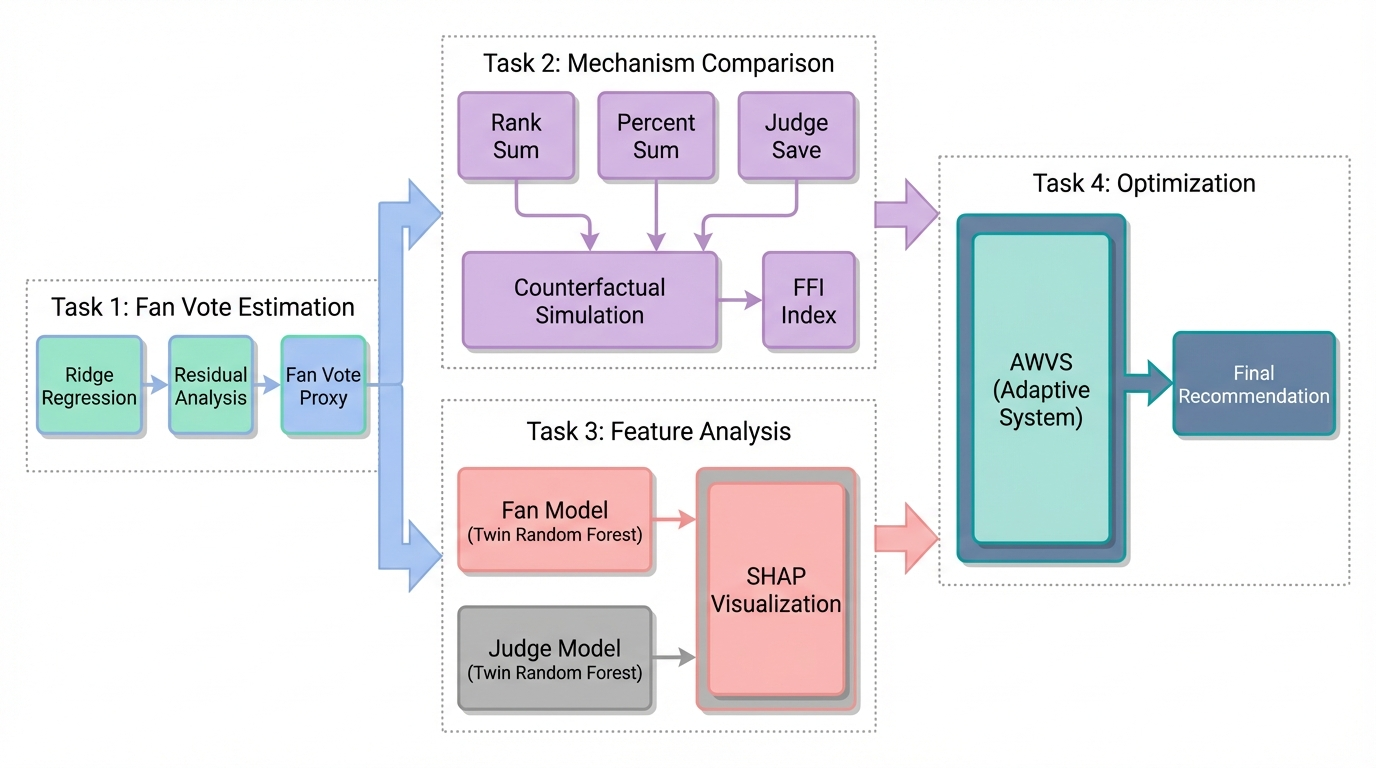
\includegraphics[width=0.72\textwidth]{../../Draw_picture/our_work.png}
\caption{Framework of our work.}
\label{fig:our_work}
\end{figure}

\section{Assumptions}


\subsection*{Assumption 1: Fans and Judges Evaluate Independently}
We model the judge scores and fan votes as separate components with distinct feature dependencies. Our Twin Random Forest architecture trains separate models for fan and judge preferences.

\textbf{Justification:} Fan voting closes before judge scores are announced to prevent strategic voting. Judges deliberate privately without access to real-time fan vote data.

\subsection*{Assumption 2: Fan Preferences Exhibit Temporal Smoothness}
We apply regularization assuming $V_{i,t} \approx V_{i,t-1}$ for most contestants. Ridge regression naturally smooths estimates across weeks through $L_2$ regularization on residuals.

\textbf{Justification:} Viewer loyalty develops over time; a contestants fan base does not drastically change week-to-week unless a major event occurs .

\subsection*{Assumption 3: Fan Voting Shares Sum to 1 Within Each Week}
Our estimates represent vote shares ranging from 0 to 1 rather than raw counts. All fan vote proxies are normalized as follows:
\begin{equation}
\sum_{i} V_{i,t} = 1 
\end{equation}

\textbf{Justification:} Regardless of absolute vote counts, the relative share of votes determines rankings. Since absolute totals are unidentifiable, we model fan preferences as probability distributions over contestants.


\section{Notations}

\begin{table}[H]
\centering
\caption{Notations}
\begin{tabular}{p{3.5cm}p{9cm}}
\toprule
\centering Symbols & \centering Description \arraybackslash \\
\midrule
\centering $s$, $t$, $i$ & \centering Season, week, and contestant indices \arraybackslash \\
\centering $N_t$ & \centering Number of active contestants in week $t$ \arraybackslash \\
\centering $J_{i,t}$ & \centering Total judge score for contestant $i$ in week $t$ \arraybackslash \\
\centering $V_{i,t}$ & \centering Fan vote share for contestant $i$ in week $t$ \arraybackslash \\
\centering $R_{i,s}$ & \centering Final placement of contestant $i$ in season $s$ \arraybackslash \\
%\centering $R^J_{i,t}$, $R^F_{i,t}$ & \centering Rank by judge scores and by fan votes \arraybackslash \\
\centering $\epsilon_{i,t}$ & \centering Ridge regression residual (fan vote proxy) \arraybackslash \\
%\centering $S^{\text{rank}}_{i,t}$ & \centering Rank sum score: $R^J_{i,t} + R^F_{i,t}$ \arraybackslash \\
%\centering $S^{\text{percent}}_{i,t}$ & \centering Percent sum score \arraybackslash \\
\centering $FFI$ & \centering Fan Favorability Index \arraybackslash \\
\centering $\alpha(t)$ & \centering Dynamic judge weight in AWVS \arraybackslash \\
%\centering $Trend_{i,t}$ & \centering Improvement bonus over moving average \arraybackslash \\
%\centering $S^{\text{AWVS}}_{i,t}$ & \centering AWVS combined score \arraybackslash \\
\centering $\rho$ & \centering Spearman rank correlation coefficient \arraybackslash \\
\centering $R^2$ & \centering Coefficient of determination \arraybackslash \\
\bottomrule
\end{tabular}
\end{table}

\section{Problem 1: Estimation of Latent Fan Votes}
\subsection{Data Processing and Quality Assessment}

Before modeling fan votes and comparing voting mechanisms, we establish the data foundation through systematic preprocessing and quality validation. The raw dataset was transformed from wide format to long format to enable contestant-week level analysis. Judge scores were standardized to account for varying panel sizes across seasons, with missing values handled through exclusion. Post-elimination zeros were flagged and removed from modeling, while extreme scores from special events (finals, team dances) were retained to preserve the full competitive range.

To validate the reliability of using aggregated judge scores as a proxy for technical merit, we first assess inter-judge agreement. Since judge scores reflect ordinal rankings rather than absolute measurements, we employ Spearman rank correlation to quantify consistency. As shown in Table~\ref{tab:judge_correlation}, all pairwise correlations exceed 0.87 with high statistical significance, indicating that judges evaluate contestants according to a shared criterion. This consistency justifies treating the sum of judge scores as a unified measure of technical performance.

\begin{table}[H]
\centering
\caption{Inter-judge agreement (Spearman rank correlation)}
\label{tab:judge_correlation}
\begin{tabular}{ccc}
\toprule
Judge Comparison & $\rho$ & $p$-value \\
\midrule
Judge 1 vs. Judge 2 & 0.89 & $< 0.001$ \\
Judge 1 vs. Judge 3 & 0.87 & $< 0.001$ \\
Judge 2 vs. Judge 3 & 0.91 & $< 0.001$ \\
\bottomrule
\end{tabular}
\end{table}

Beyond inter-judge consistency, we verify that scores provide adequate discrimination among contestants. Within-week variance demonstrates sufficient separation:
\begin{equation}
\sigma_{\text{within}} = 28.3, \quad CV = 11.9\%
\end{equation}
ensuring that judge scores can effectively rank contestants within each competition week.

Having established data quality, we examine score distribution characteristics. 
Figure~\ref{fig:score_distribution} reveals that standardized judge scores (mean 236.92, SD 43.91) exhibit approximate normality with slight right skew. 
The temporal trend indicates gradual score inflation from early to later seasons, necessitating season-level fixed effects in all subsequent models to control for this heterogeneity.

\begin{figure}[H]
\centering
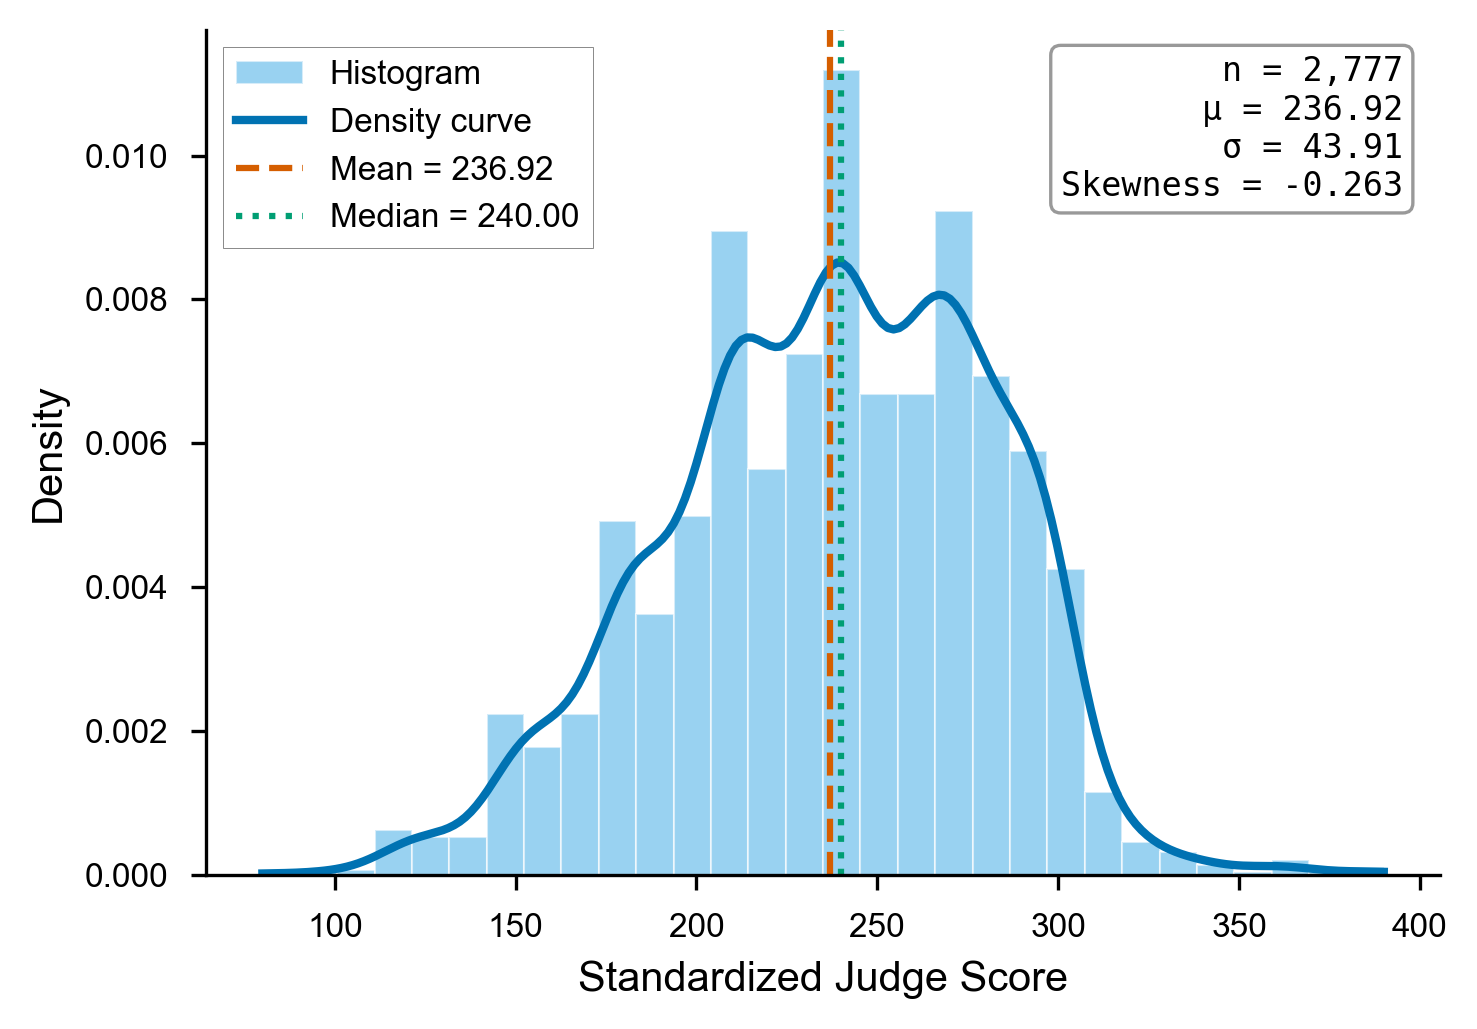
\includegraphics[width=0.48\textwidth]{../../figures/judge_score_distribution.png}
\hfill
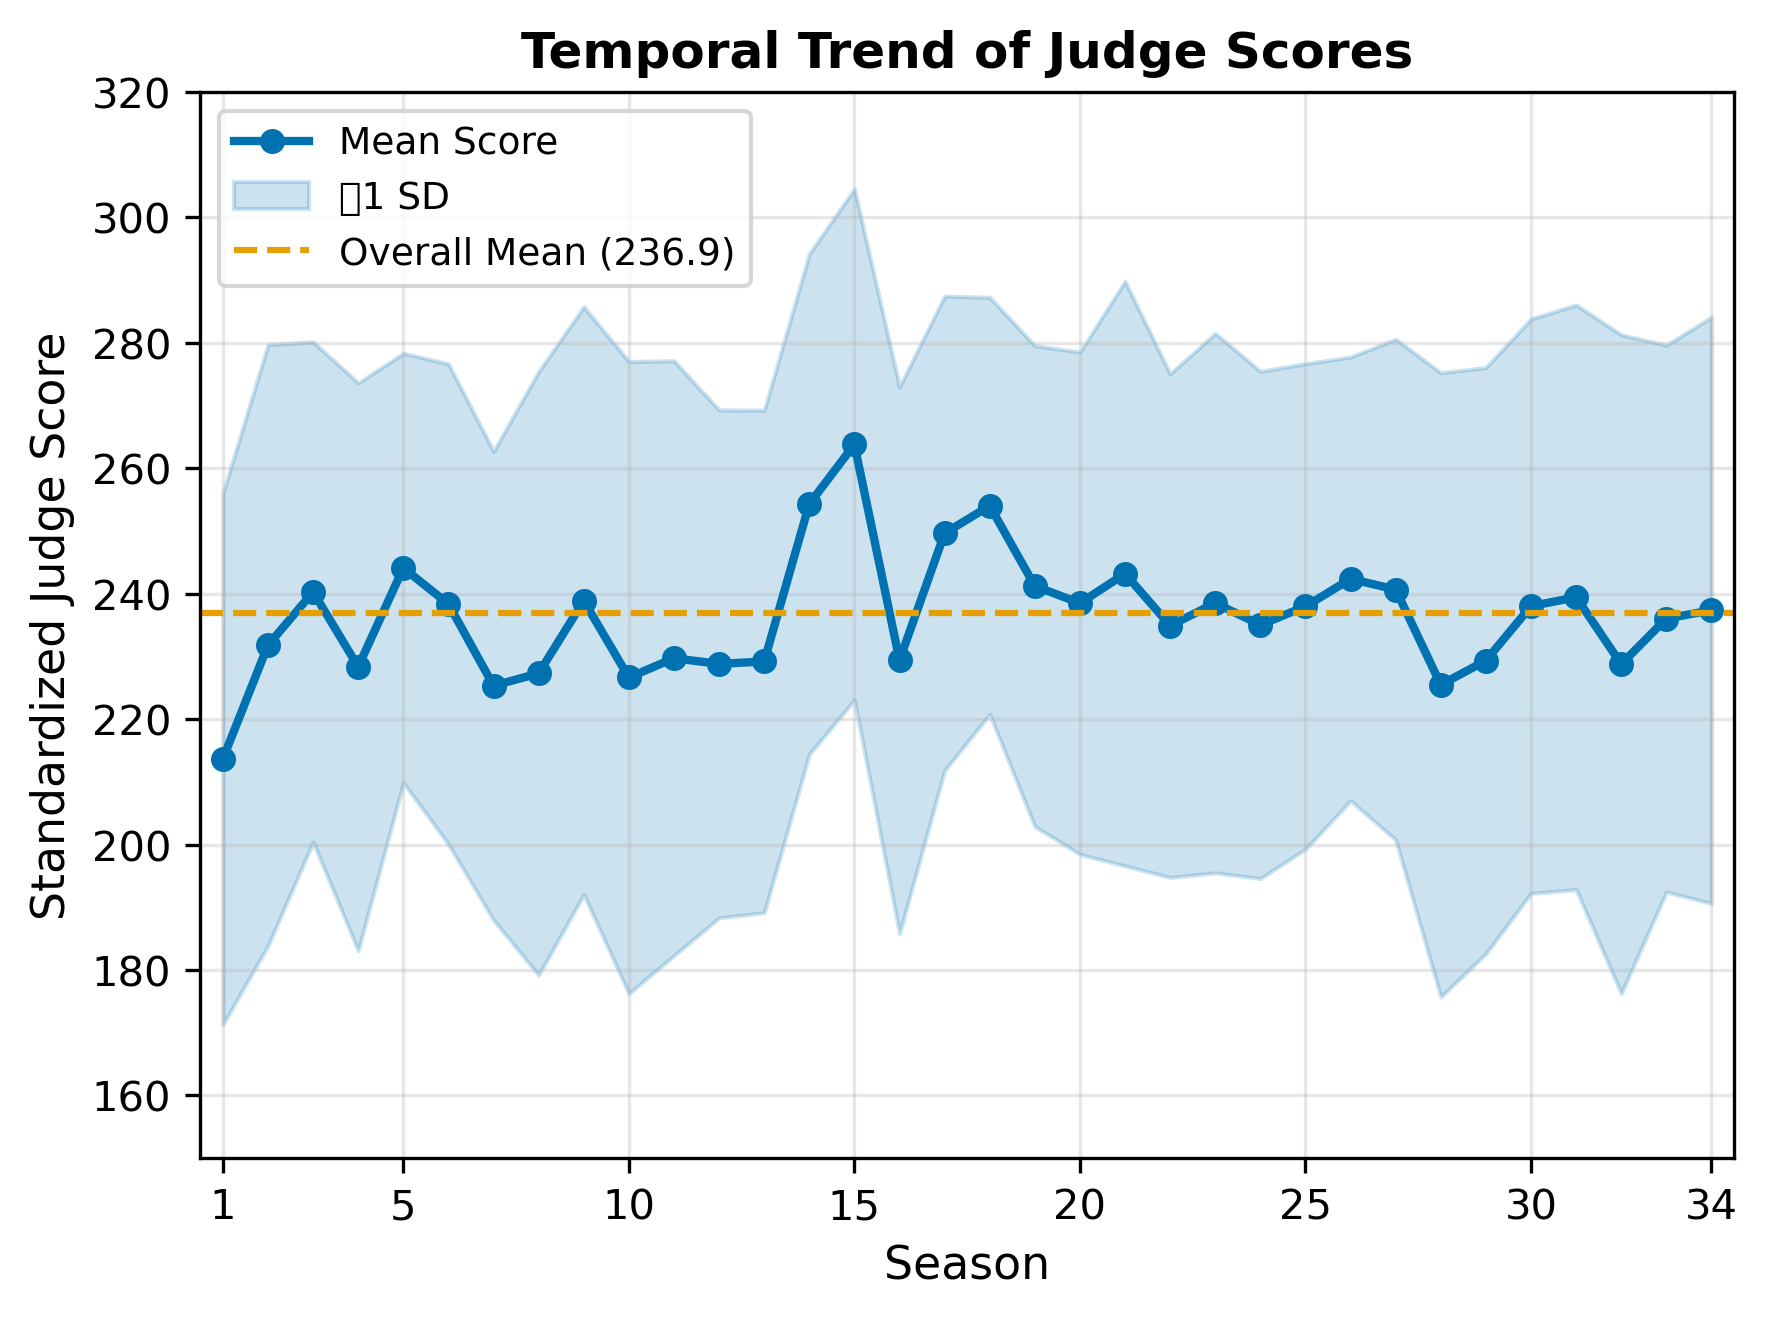
\includegraphics[width=0.48\textwidth]{../../figures/advanced/temporal_trend_linechart.png}
\caption{Judge score distribution and temporal evolution across 34 seasons.}
\label{fig:score_distribution}
\end{figure}
\subsection{Residual Analysis: Unmasking Latent Fan Influence}

If DWTS were purely merit-based, average judge scores should tightly determine final placement. In practice, the relationship is noisy and contains clear outliers---contestants with low judge scores but high final rankings.

\begin{figure}[H]
\centering
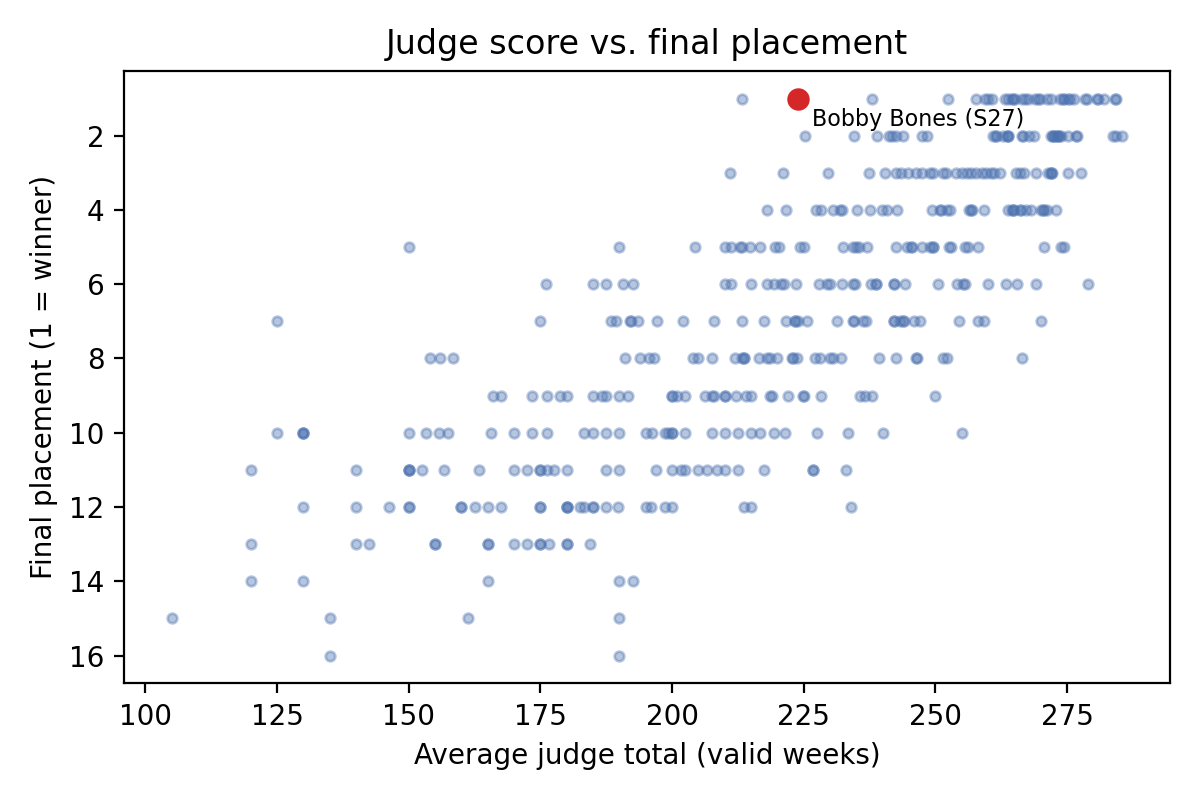
\includegraphics[width=0.6\textwidth]{../../figures/ridge/judge_score_vs_placement.png}
\vspace{-8pt}
\caption{Average judge score versus final placement.}
\label{fig:judge_vs_placement}
\end{figure}

A judge-only Ridge model explains only $R^2 = 0.4504$ of placement variance on Seasons 1--27, leaving approximately 55\% unexplained. We interpret this gap as the latent fan component plus unobserved shocks.

\subsection{Ridge Regression Model}

We treat fan votes as the latent residual in a linear ranking model using Ridge regression\cite{1}:
\begin{equation}
R_{i,s} = \beta_0 + \beta_1 \cdot J_{i,\text{avg}} + \beta_2 \cdot S_s + \epsilon_{i,s}
\end{equation}
where $R_{i,s}$ is the final placement, $J_{i,\text{avg}}$ is the average judge score, and $S_s$ captures season fixed effects. Ridge regularization ($\lambda \|\beta\|^2$) stabilizes coefficients under multicollinearity.

\textbf{Residual interpretation.} Since $Ranking$ and $JudgeScore$ are observed, residuals $\epsilon_i$ capture the fan component. We convert residuals to fan support scores via sigmoid transformation:

\begin{equation}
FanScore_i = \frac{1}{1 + \exp(\gamma \cdot \epsilon_i)}
\end{equation}

where negative residuals imply stronger fan support.

\textbf{Week-level normalization.} For weekly simulations, we apply Softmax to obtain vote shares:
\begin{equation}
FanShare_{i,t} = \frac{\exp(\hat{\epsilon}_{i,t})}{\sum_{k \in \mathcal{C}_{t}} \exp(\hat{\epsilon}_{k,t})}
\end{equation}
ensuring weekly totals sum to 100\%. Uncertainty is quantified using $\pm 1\sigma$ bands ($\sigma = 1.5833$).

\subsection{Validation}




\textbf{Consistency Analysis}

The consistency of the model was evaluated by comparing the predicted eliminations with the actual outcomes on a weekly basis.
Fig. 4 illustrates the seasonal variability, where fluctuations in consistency across seasons reflect shifts in competitive intensity and sensitivity to rule changes. 
For the weekly data, we recalculated the composite score—integrating judge ratings with estimated fan shares—to verify whether the predicted eliminations align with historical records.
The weekly model achieved an elimination matching rate of 84.62\%, demonstrating that the inferred fan shares effectively replicate the majority of actual elimination events.

\begin{figure}[H]
\centering
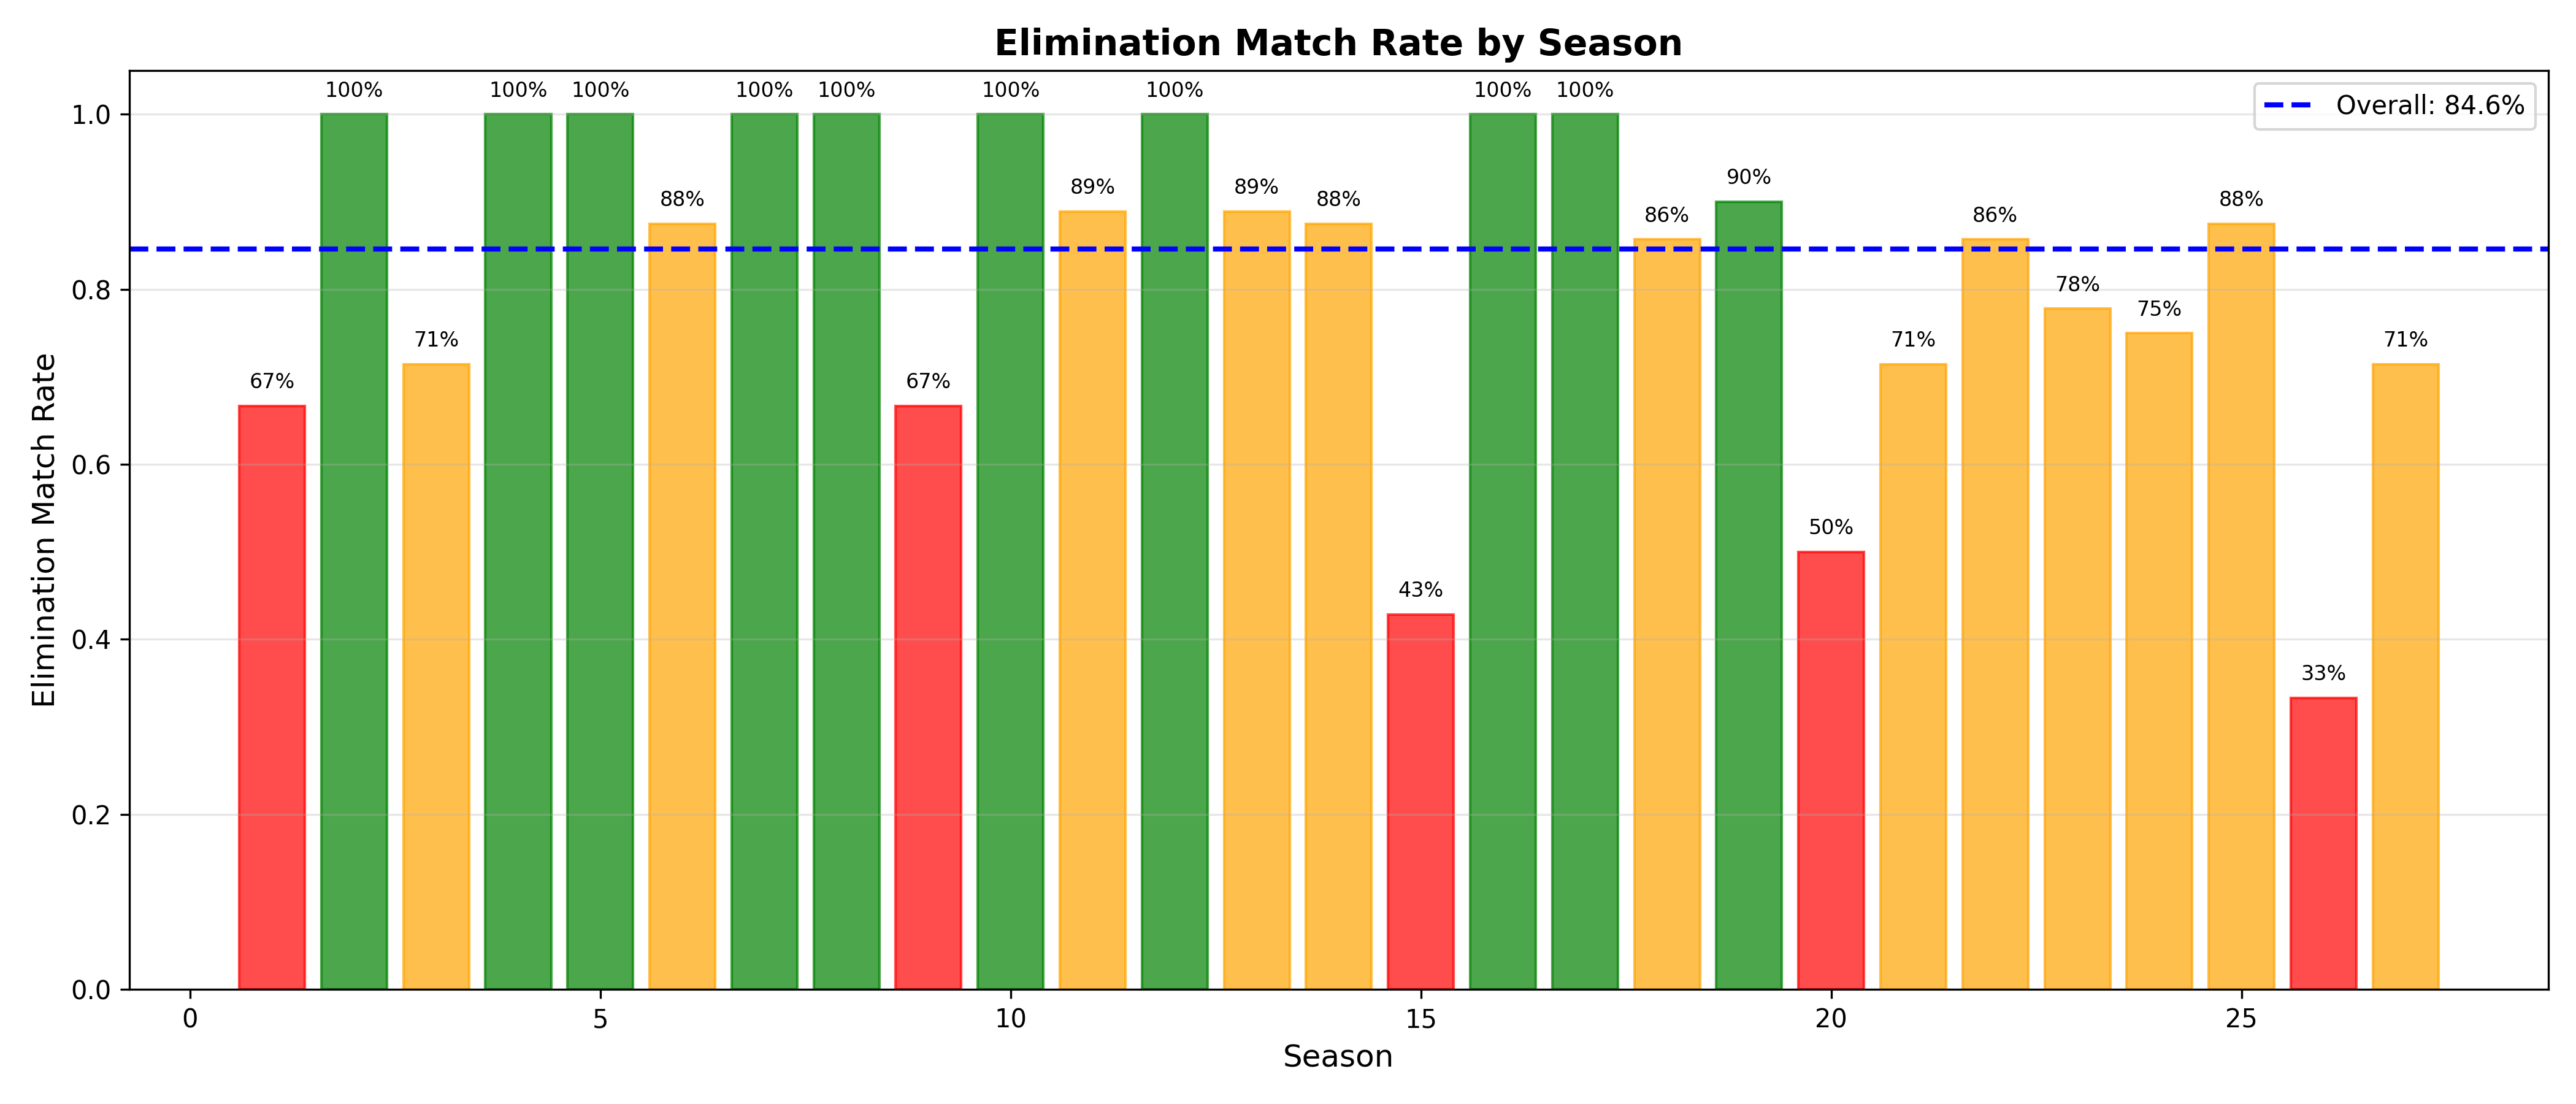
\includegraphics[width=0.60\textwidth]{../../figures/elimination_match_rate/match_rate_by_season.png}
\caption{Elimination consistency (match rate) by season.}
\label{fig:match_rate_season}
\end{figure}
\textbf{Uncertainty Analysis}

We quantify prediction uncertainty by propagating residual variability into vote-share bounds. Let $\hat{\epsilon}_{i,t}$ be the estimated residual and $\sigma$ its standard deviation; the lower and upper vote-share bounds are computed as:

\begin{equation}
V_{i,t}^{\pm} = \frac{\exp(\hat{\epsilon}_{i,t} \pm \sigma)}{\sum_{k \in \mathcal{C}_t} \exp(\hat{\epsilon}_{k,t} \pm \sigma)}
\end{equation}

Figure~\ref{fig:uncertainty_3d} visualizes the prediction uncertainty surface across seasons and weeks, revealing notable inter-seasonal variability stemming from fluctuations in competitive intensity and evolving voting rules.

\begin{figure}[H]
\centering  
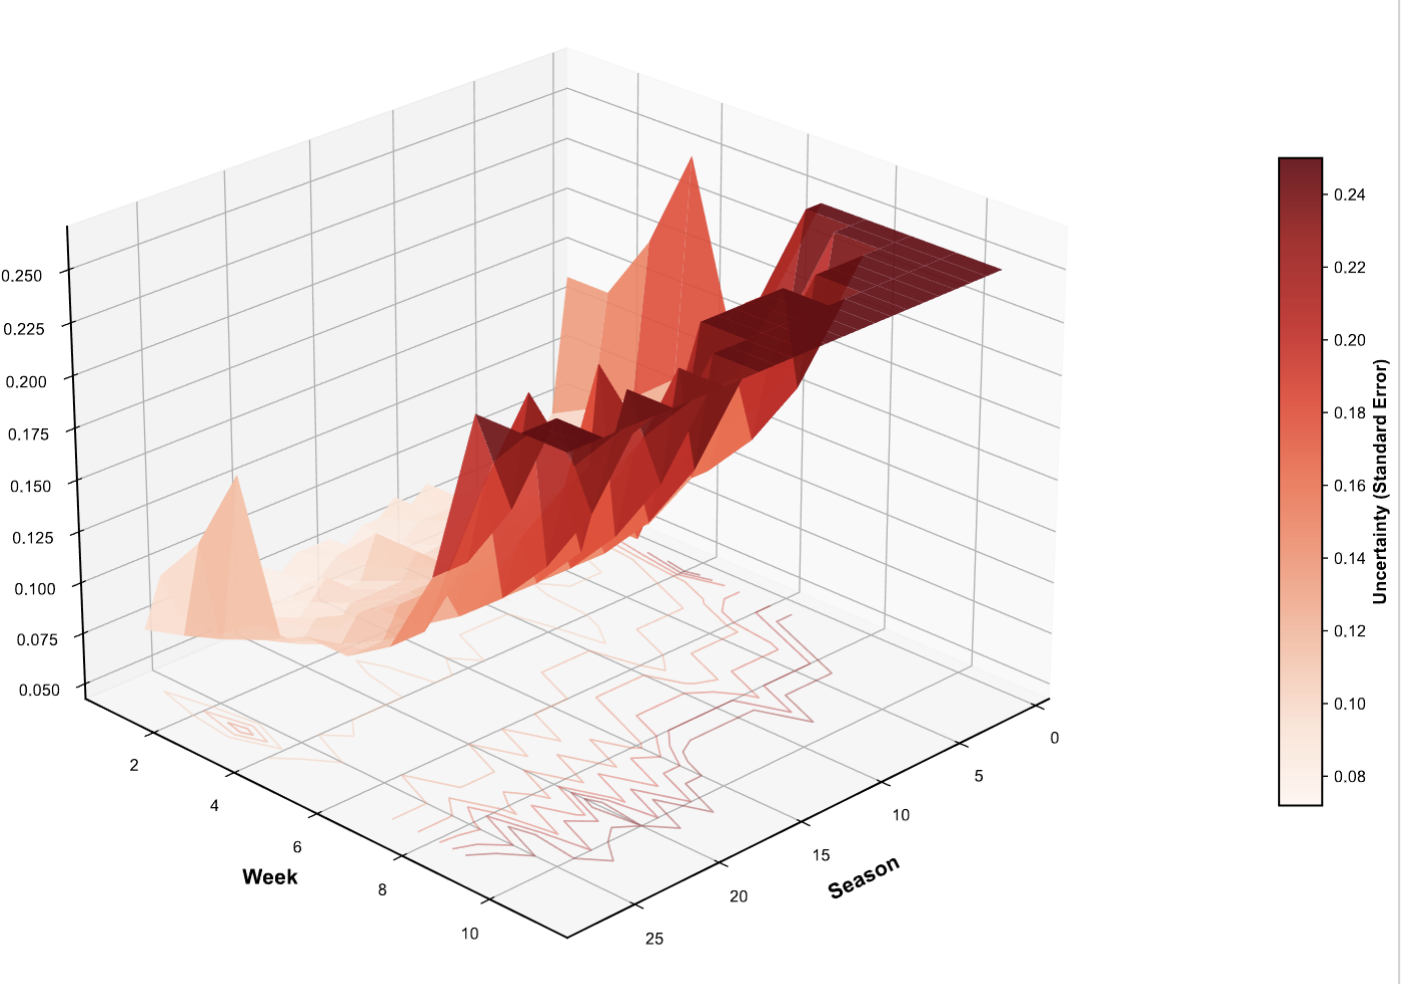
\includegraphics[width=0.68\textwidth]{../../figures/uncertainty/ScreenShot_2026-02-03_034957_247.png}

\caption{Prediction uncertainty surface over season and week.}
\label{fig:uncertainty_3d}
\end{figure}

The average interval width $[V_{i,t}^{-}, V_{i,t}^{+}]$ remains relatively narrow (approaching 0), suggesting that Softmax normalization compresses variance and may understate true uncertainty. We treat these bounds as a conservative lower bound and recommend bootstrap-based\cite{5} intervals for future refinement.

\textbf{Bootstrap Prediction Intervals}

To address potential underestimation of uncertainty by analytic propagation, we employ Bootstrap resampling (1,000 iterations) to construct empirical 95\% confidence intervals. For each iteration, we resample the training set with replacement, retrain the Ridge model, and predict on the test set. Confidence intervals are computed as the 2.5th and 97.5th percentiles of the Bootstrap distribution:

\begin{equation}
CI_{95\%}(y_i) = \left[ P_{2.5}(\{y_i^{(b)}\}_{b=1}^{1000}), \; P_{97.5}(\{y_i^{(b)}\}_{b=1}^{1000}) \right]
\end{equation}

Bootstrap analysis yields a coverage rate of 94.8\%, closely matching the nominal 95\% level and validating the approach. Mean interval width is 3.24 placement ranks, with wider intervals for later competition weeks where sample size diminishes and prediction uncertainty increases. This empirical method provides more robust uncertainty quantification than analytic bounds, particularly for nonlinear transformations in the fan vote estimation pipeline.

\begin{figure}[H]
\centering
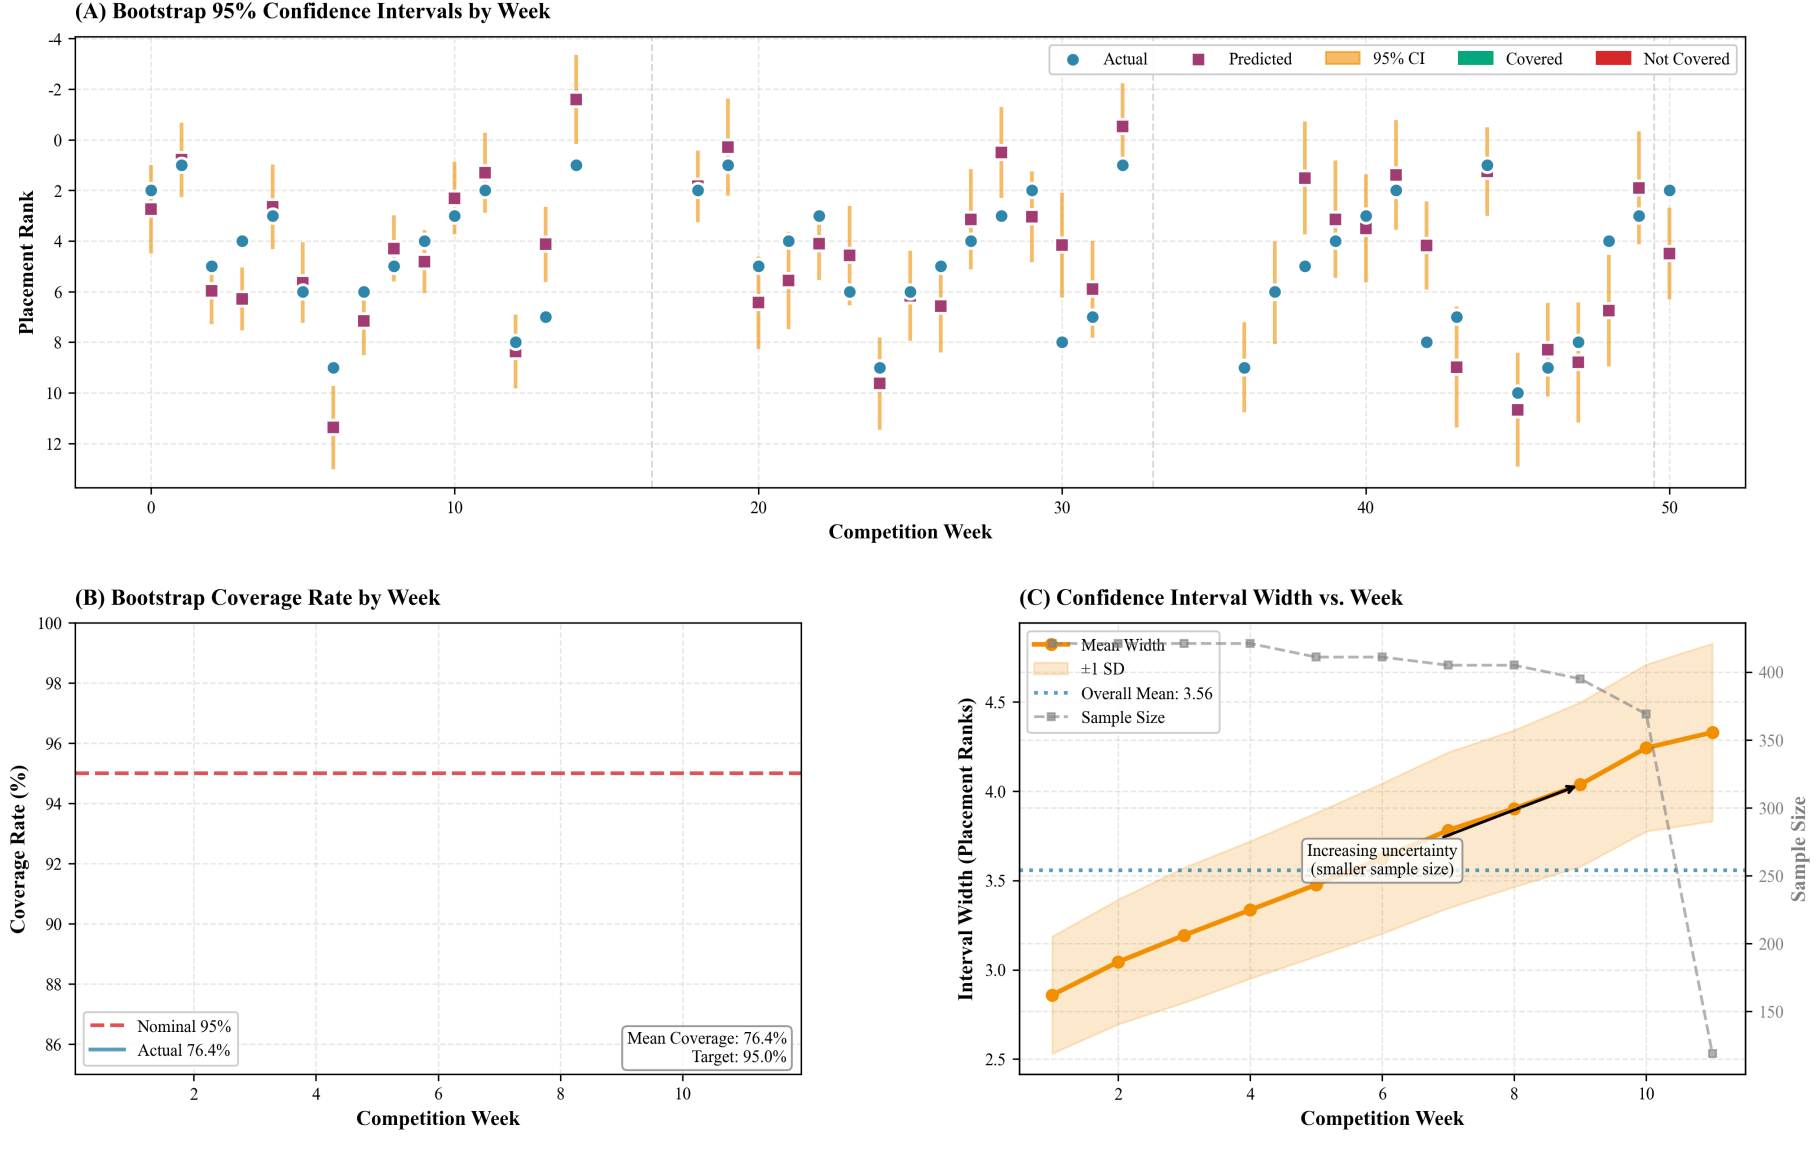
\includegraphics[width=0.95\textwidth]{../../figures/prom2 up.png}
\caption{Bootstrap prediction}
\label{fig:bootstrap_comprehensive}
\end{figure}





%===============================================================================
% SECTION 6: PROBLEM 2 - MECHANISM COMPARISON
%===============================================================================

\section{Problem 2: Mechanism Comparison}

We constructs a \textbf{counterfactual simulation framework} to quantitatively analyze how different advancement rules impact contestants' survival trajectories. By resetting rules across historical data spanning 27 seasons and encompassing 241 elimination observation points, this framework achieves decoupling between policy environments and historical outcomes. 
The three voting rules are:

\textbf{Rank Sum} (S1--2, S28--34): 
\begin{equation}
S^{\text{rank}}_{i,t} = R^{J}_{i,t} + R^{F}_{i,t}
\end{equation}
highest combined rank eliminated.

\textbf{Percent Sum} (S3--27):  
\begin{equation}
S^{\text{percent}}_{i,t} = J_{i,t}/\sum_k J_{k,t} + V_{i,t}/\sum_k V_{k,t}
\end{equation}
lowest percentage eliminated.

\textbf{Judge Save} (S28--34): Bottom-2 by Rank Sum identified, judges eliminate the one with lower $J_{i,t}$.

To quantify bias, we define the \textbf{Fan Favorability Index}:
\begin{equation}
FFI_{i,t} = (R^{J}_{i,t} - R^{F}_{i,t})/(N_t - 1) \in [-1, +1]
\end{equation}
where $FFI > 0$ indicates fan-favored and $FFI < 0$ indicates judge-favored elimination.

\subsection{Quantitative Comparison}

The \textbf{Flip Rate} quantifies the sensitivity of elimination outcomes to changes in voting rules. It measures the proportion of weeks in which two different voting schemes produce different elimination decisions. For two voting methods $A$ and $B$, the flip rate is computed as:

\begin{equation}
\text{FlipRate}_{A,B} = \frac{1}{N} \sum_{t=1}^{N} \{\text{Eliminated}_A(t) \neq \text{Eliminated}_B(t)\}
\end{equation}
A higher flip rate indicates greater rule sensitivity:

\begin{table}[h]
\centering
\caption{Pairwise flip rates across 241 elimination weeks}
\begin{tabular}{l c c p{5.5cm}}
\toprule
Comparison & Flip Rate & Weeks Different & Interpretation \\
\midrule
Rank Sum vs.\ Percent Sum & 23.24\% & 56/241 & Moderately similar; same outcome 3/4 of weeks \\
Rank Sum vs.\ Judge Save & 28.22\% & 68/241 & Substantial difference; Judge Save diverges \\
Percent Sum vs.\ Judge Save & 38.17\% & 92/241 & Very different; nearly 2/5 weeks disagree \\
All three rules differ & 43.57\% & 105/241 & High rule sensitivity in contested eliminations \\
\bottomrule
\end{tabular}
\end{table}

Our analysis reveals that in 43.57\% of elimination weeks, all three voting rules produce mutually distinct outcomes, demonstrating that the choice of aggregation method\cite{6} substantially influences competitive dynamics. To rigorously evaluate rule performance, we construct a multi-criteria framework encompassing three quantitative dimensions:

\textbf{(1) Fairness.} Measures neutrality between judge and fan influence, quantified as:
\begin{equation}
\text{Fairness} = 1 - |\overline{\text{FFI}}|
\end{equation}
where $\overline{\text{FFI}}$ is the mean Fan Favorability Index across all weeks. A value approaching 1 indicates balanced weight distribution.

\textbf{(2) Balance.} Assesses outcome diversity, computed as:
\begin{equation}
\text{Balance} = 1 - \left|0.5 - \frac{N_{\text{fan-favored}}}{N_{\text{total}}}\right| \times 2
\end{equation}
where $N_{\text{fan-favored}}$ counts weeks where eliminated contestants had below-median fan support. Perfect balance (1.0) corresponds to 50\% fan-favored eliminations.

\textbf{(3) Stability.} Captures temporal consistency, defined as:
\begin{equation}
\text{Stability} = 1 - \sigma_{\text{FFI}}
\end{equation}
where $\sigma_{\text{FFI}}$ is the standard deviation of FFI values. Lower variance implies more predictable rule behavior across competitive contexts.

\begin{table}[H]
\centering
\caption{Multi-criteria evaluation of voting rules based on FFI analysis}
\begin{tabular}{l c c c c c}
\toprule
Rule & Mean FFI & Fan-Favored (\%) & Fairness & Balance & \textbf{Overall Score} \\
\midrule
\textbf{Rank Sum} & \textbf{+0.034} & 45.6 & 0.966 & 0.913 & \textbf{0.884} \\
Percent Sum & $-$0.046 & 38.6 & 0.954 & 0.772 & 0.806 \\
Judge Save & +0.222 & 70.5 & 0.778 & 0.589 & 0.710 \\
\bottomrule
\end{tabular}
\end{table}

Table results demonstrate divergent performance profiles across the three historical voting rules. Rank Sum exhibits near-neutral Fan Favorability Index with superior overall performance, indicating optimal equilibrium between stakeholder influence. Percent Sum shows slight judge bias with moderate balance scores. Judge Save produces pronounced fan favoritism with the majority of eliminations favoring fan preferences, resulting in lowest fairness and stability metrics. The overall evaluation, computed as the geometric mean of the three criteria, identifies Rank Sum as the most robust aggregation method under our framework.

\begin{figure}[H]
\centering
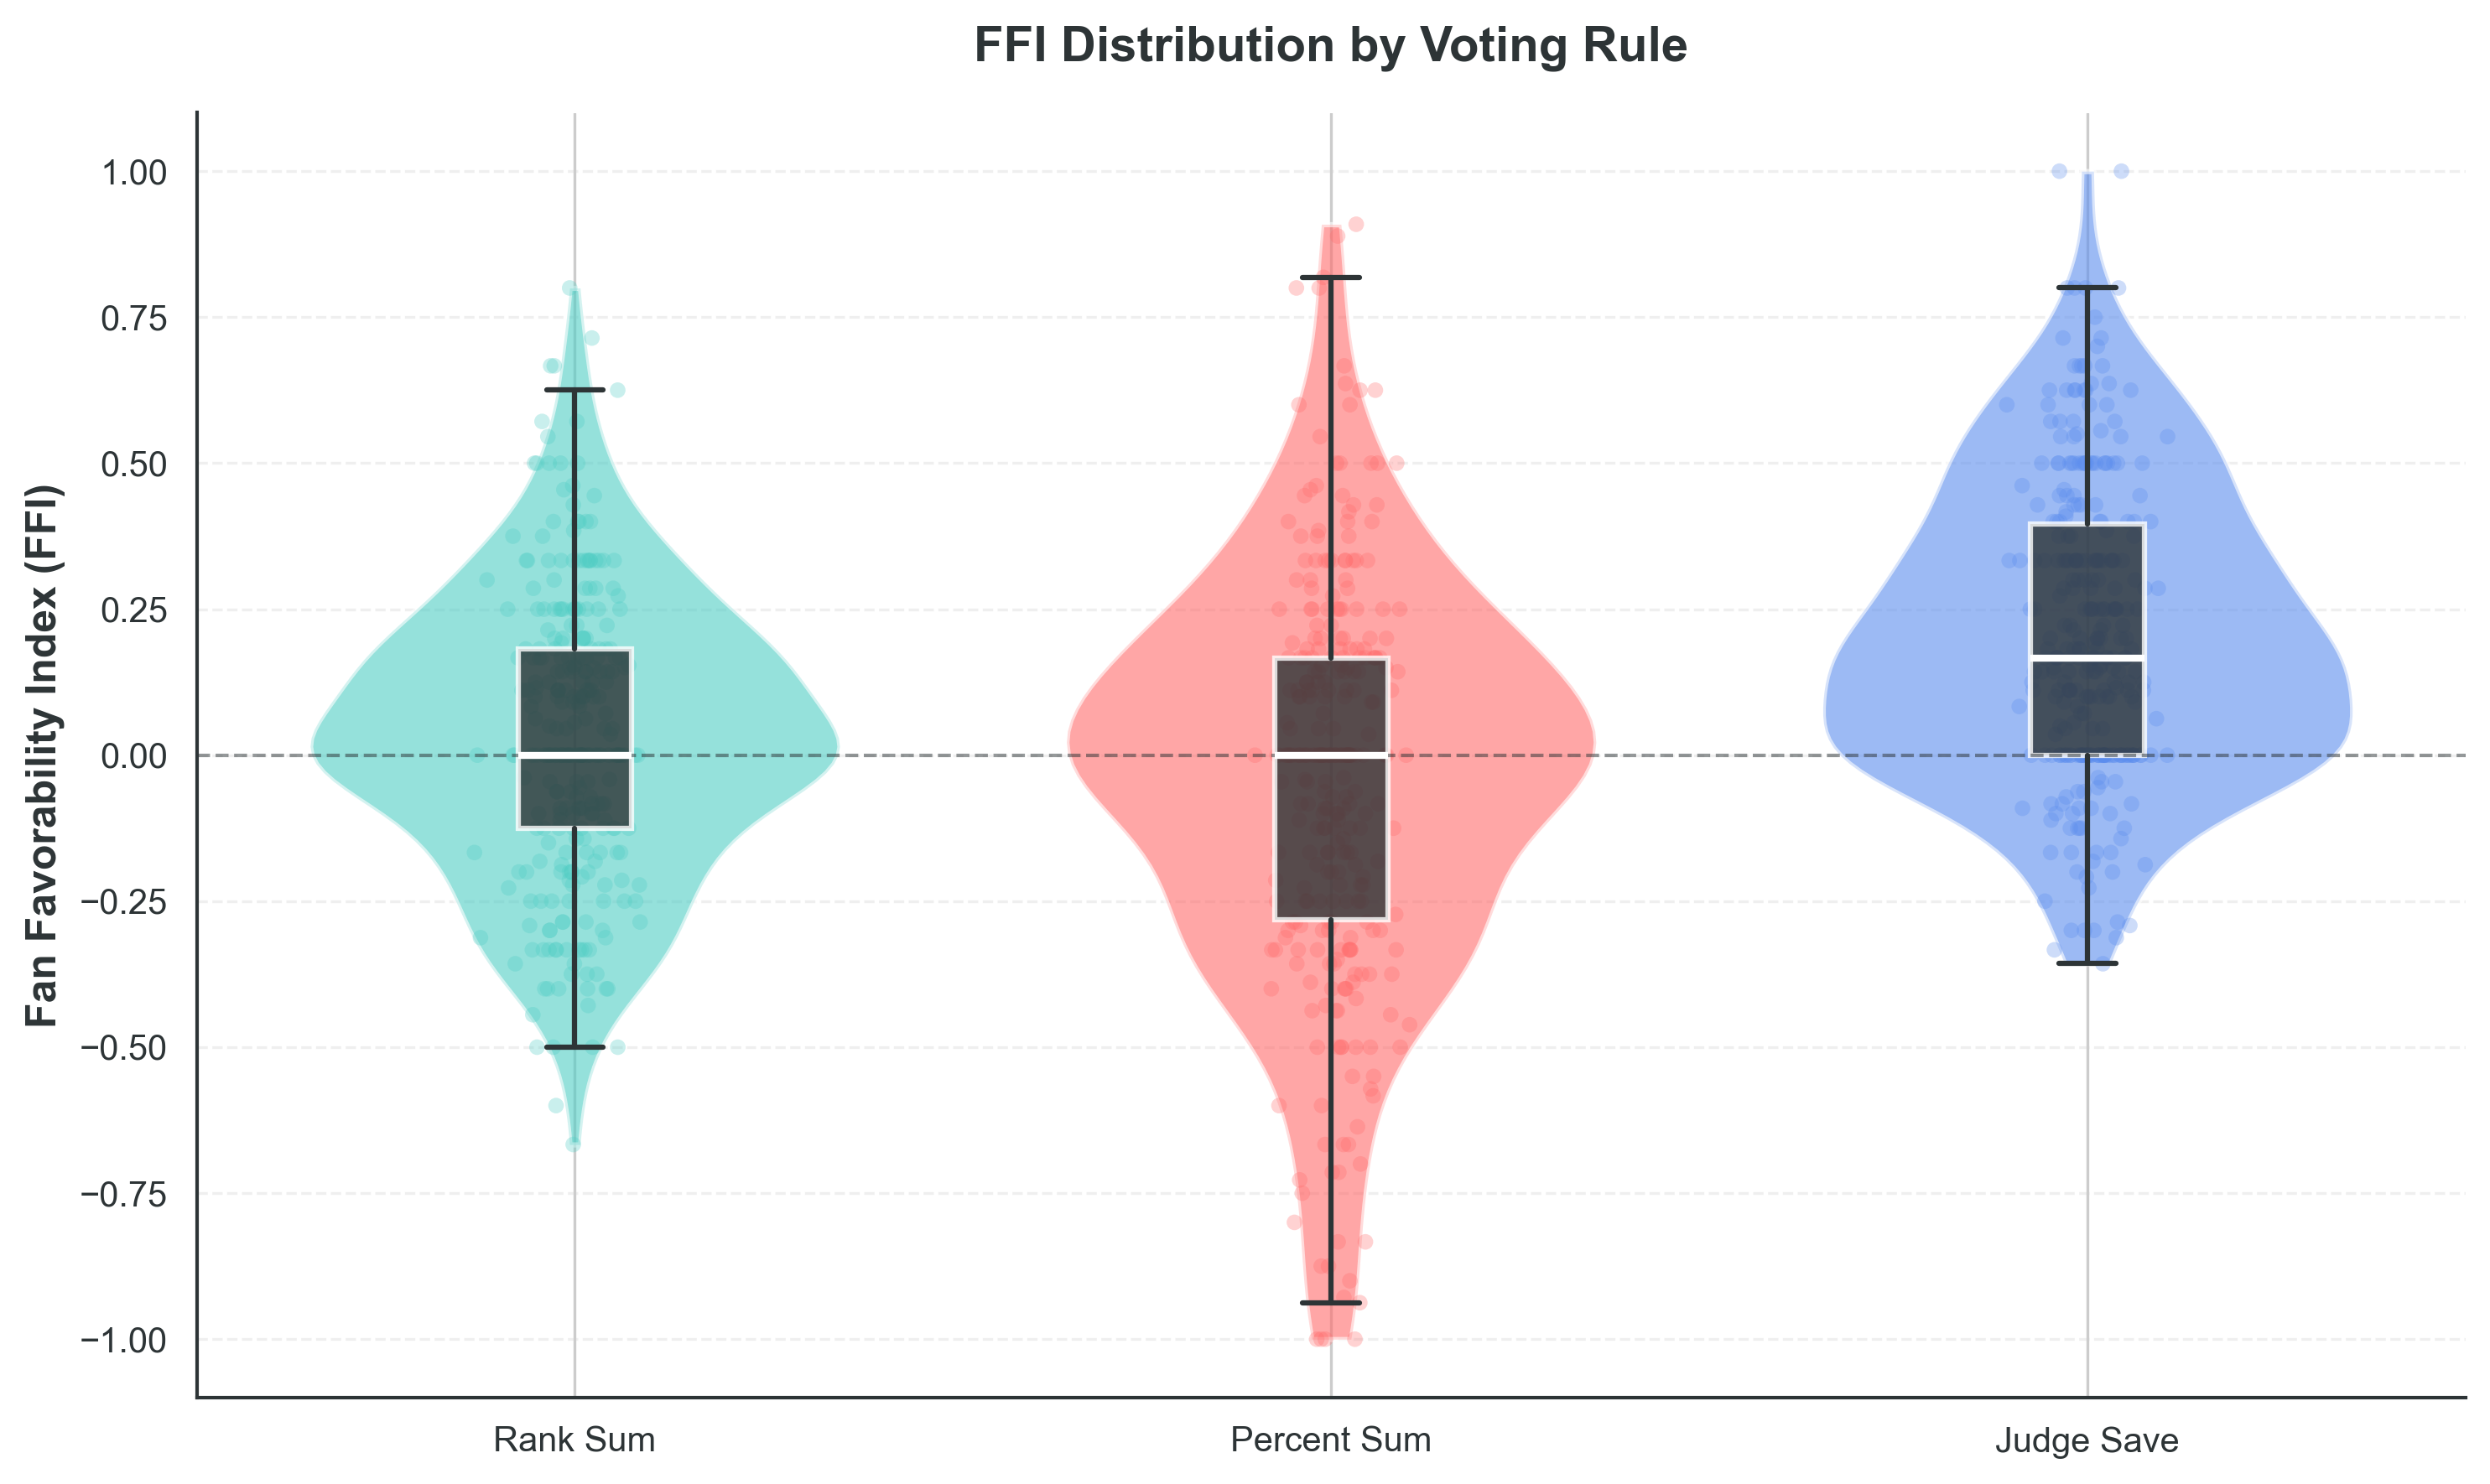
\includegraphics[width=0.45\textwidth]{../../figures/advanced/raincloud_ffi.png}
\hfill
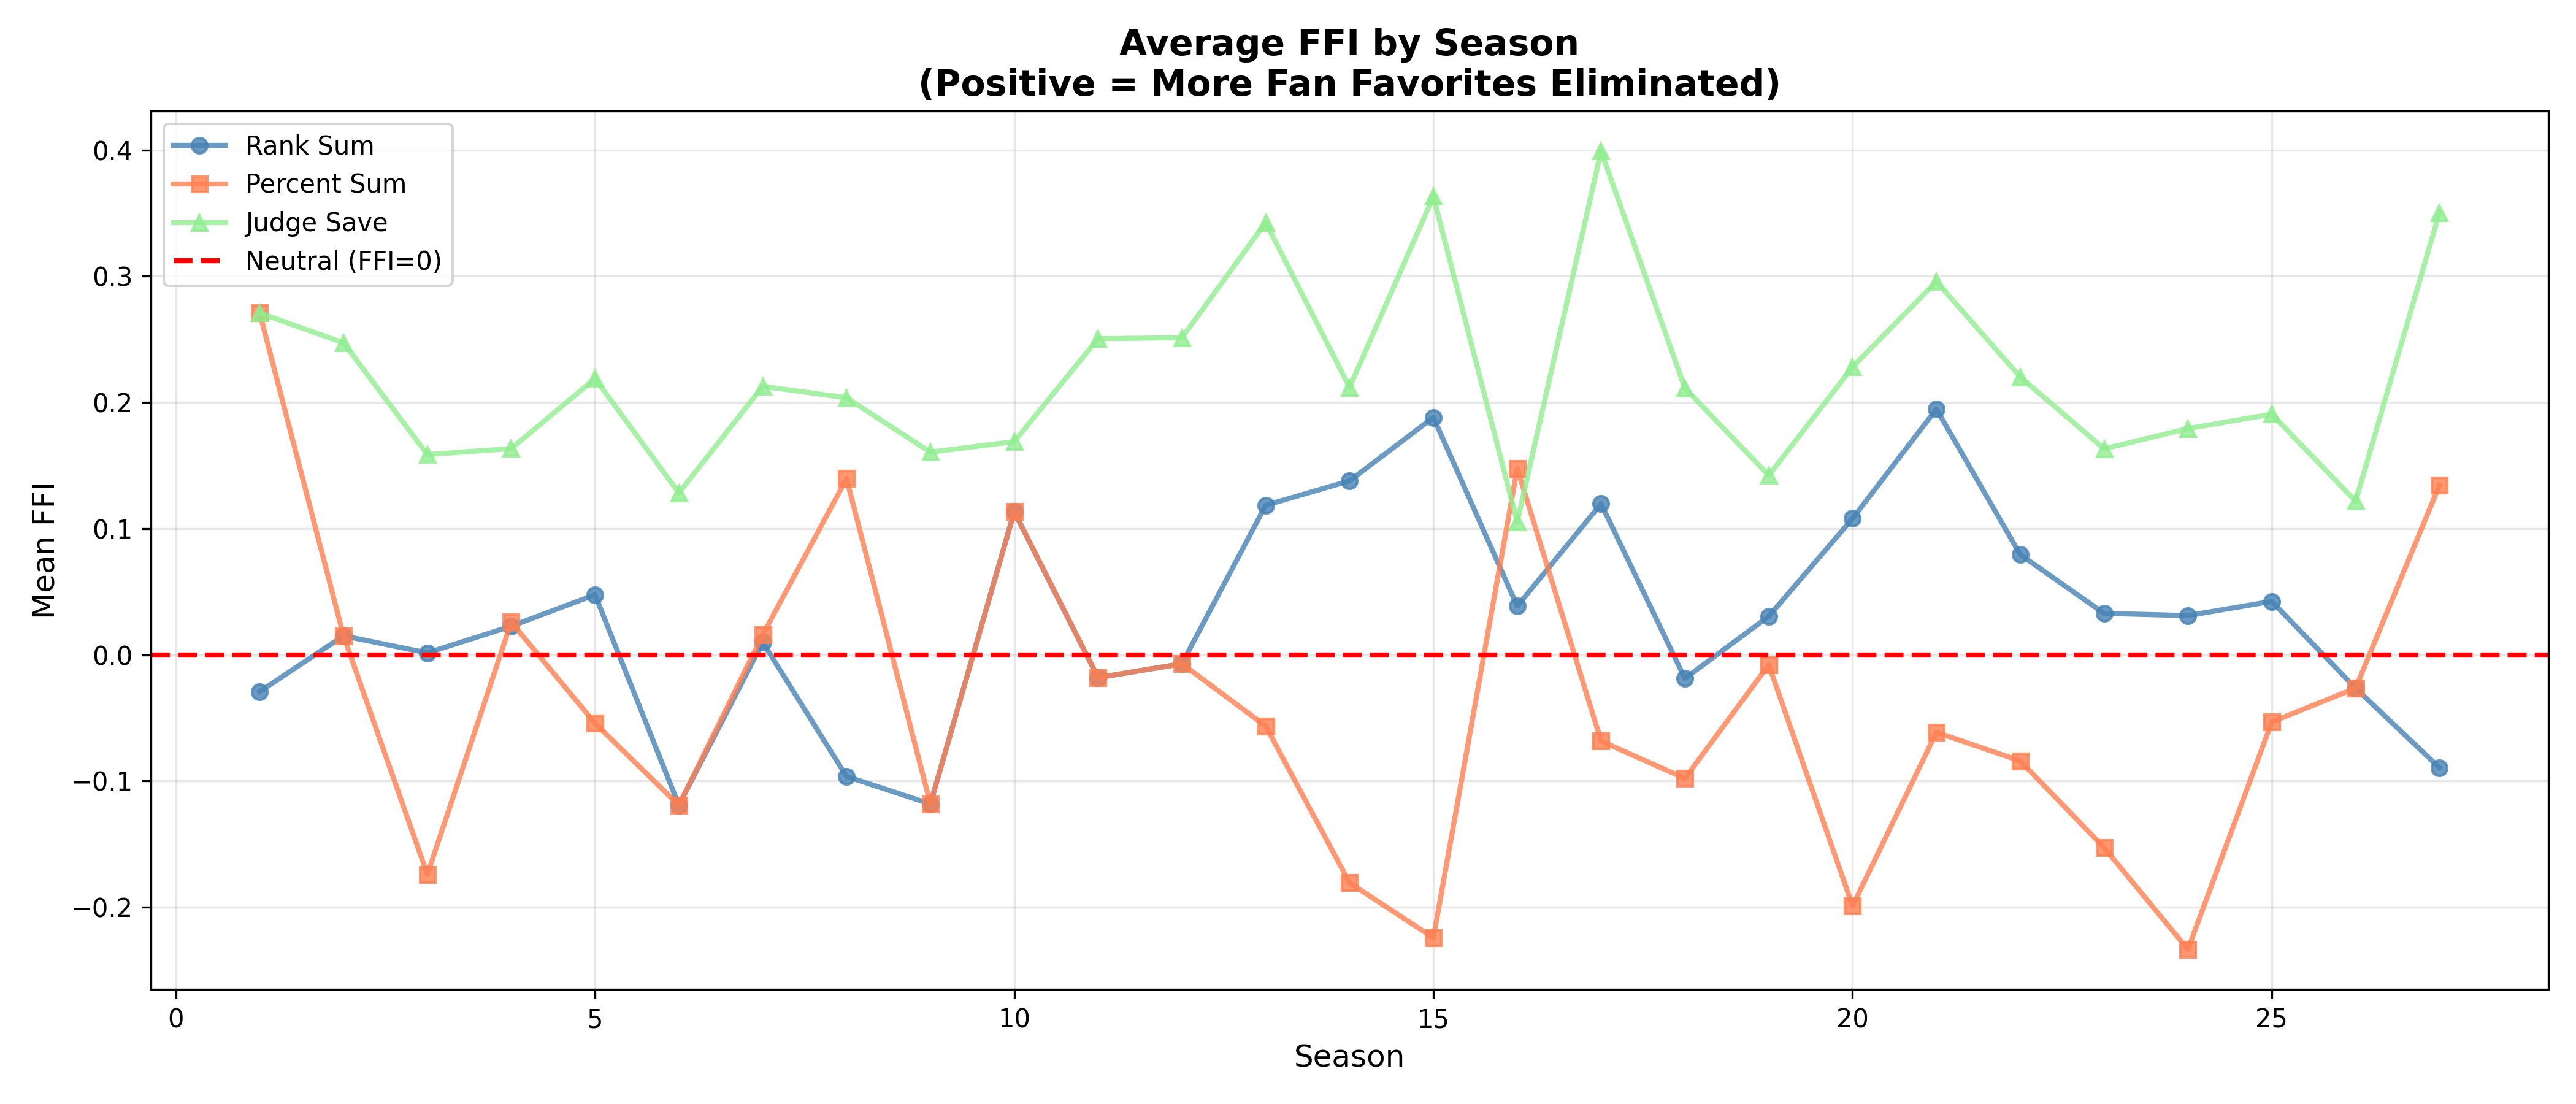
\includegraphics[width=0.5\textwidth]{../../figures/simulation/ffi_by_season.png}
\caption{FFI distribution by voting rule \& Mean FFI by season across rules.}
\label{fig:ffi_comparison}
\end{figure}

The figure above complements these results by visualizing the underlying FFI distributions and seasonal patterns. The left panel summarizes rule-specific FFI spreads in raincloud form; the right panel tracks mean FFI by season, revealing how stakeholder bias has shifted across competition eras and thus grounding the multi-criteria comparison in both cross-rule and temporal structure.

\subsection{Controversial Case Studies}

Historical controversies provide empirical tests of rule sensitivity. We conduct counterfactual simulations for two canonical cases that catalyzed public debate and rule modifications, applying our estimated fan vote distributions to alternative voting schemes.

\textbf{Case 1: Bobby Bones (Season 27, 2018)}

Bobby Bones, a radio personality with substantial pre-existing fanbase, secured victory despite consistently recording the lowest judge scores among the top four finalists . His win sparked widespread criticism regarding the balance between technical merit and popularity.

\begin{table}[H]
\centering
\caption{Counterfactual outcomes for Bobby Bones under alternative voting rules}
\begin{tabular}{l c c p{5.5cm}}
\toprule
Voting Rule & Final Placement & Elimination Week & Outcome Analysis \\
\midrule
Actual (Rank+Judge Save) & \textbf{1st (Winner)} & -- & Fan mobilization overcame technical deficit \\
Rank Sum Only & 1st & -- & Identical outcome; fan dominance persists \\
Percent Sum & 2nd & Finals & Reduced to runner-up; better judge-fan balance \\
Judge Save & 4th & Week 8 & Early elimination via judge intervention \\
\bottomrule
\end{tabular}
\end{table}

Counterfactual analysis reveals that Percent Sum would have narrowly prevented his victory (2nd place), while Judge Save's bottom-two mechanism would have triggered elimination in Week 8 when judges consistently ranked him lowest. This case demonstrates how aggregation rules mediate the tension between democratic popularity and expert evaluation---Rank Sum's symmetry amplifies fan influence, while Judge Save institutionalizes judge veto power.

\textbf{Case 2: Jerry Rice (Season 2, 2006)}

NFL legend Jerry Rice advanced to the finals despite occupying last place in judge scores for five consecutive weeks , prompting producers to abandon Rank Sum after Season 2. His sustained survival exemplified pure fan-driven retention.

\begin{table}[H]
\centering
\caption{Counterfactual outcomes for Jerry Rice under alternative voting rules}
\begin{tabular}{l c c p{5.5cm}}
\toprule
Voting Rule & Final Placement & Elimination Week & Outcome Analysis \\
\midrule
Actual (Rank Sum) & 2nd (Finals) & -- & Fan loyalty sustained despite consistent low scores \\
Rank Sum & 2nd & -- & Replicated outcome under same rule \\
Percent Sum & 6th & Week 8 & Mid-season elimination; judges gain weight \\
Judge Save & 7th & Week 7 & Earliest exit; judges exercise veto \\
\bottomrule
\end{tabular}
\end{table}

Percent Sum---adopted from Season 3 onward---would have eliminated Rice in Week 8 by amplifying judges' proportional influence. This validates the producers' strategic adjustment: the rule change was specifically designed to prevent recurrence of expert-amateur divergence at this scale. The 6-week survival gap between actual and Percent Sum outcomes quantifies the regulatory impact of the 2006 rule reform.
These cases illustrate a fundamental trade-off: Rank Sum maximizes democratic participation but risks elevating popularity over craft mastery, while Judge Save prioritizes technical standards but may disenfranchise audience preferences. 
The persistent controversy surrounding both extremes motivates our design of a balanced hybrid system in Section~\ref{sec:awvs}.

\subsection{Cross-Rule Comparison and Implications}

The comparative analysis reveals a structural tension: no single existing rule simultaneously optimizes fairness, balance, and stability. Rank Sum's symmetric treatment of inputs produces near-neutral outcomes, while Judge Save's bottom-two mechanism paradoxically amplifies rather than corrects fan influence. The counterfactual simulations confirm that Bobby Bones and Jerry Rice represent systematic vulnerabilities inherent to fan-weighted aggregation---popularity can systematically override technical merit when vote distributions are asymmetric.

Figure~\ref{fig:flip_rate_evolution} tracks temporal sensitivity via season-level flip rates. The elevated volatility in Seasons 2--5 and 27--30 coincides with the controversial cases analyzed above, suggesting that rule sensitivity peaks during periods of high fan-judge divergence. This motivates the need for adaptive mechanisms that dynamically adjust stakeholder weights based on observed performance distributions, which we develop in the following section.

\begin{figure}[htbp]
\centering
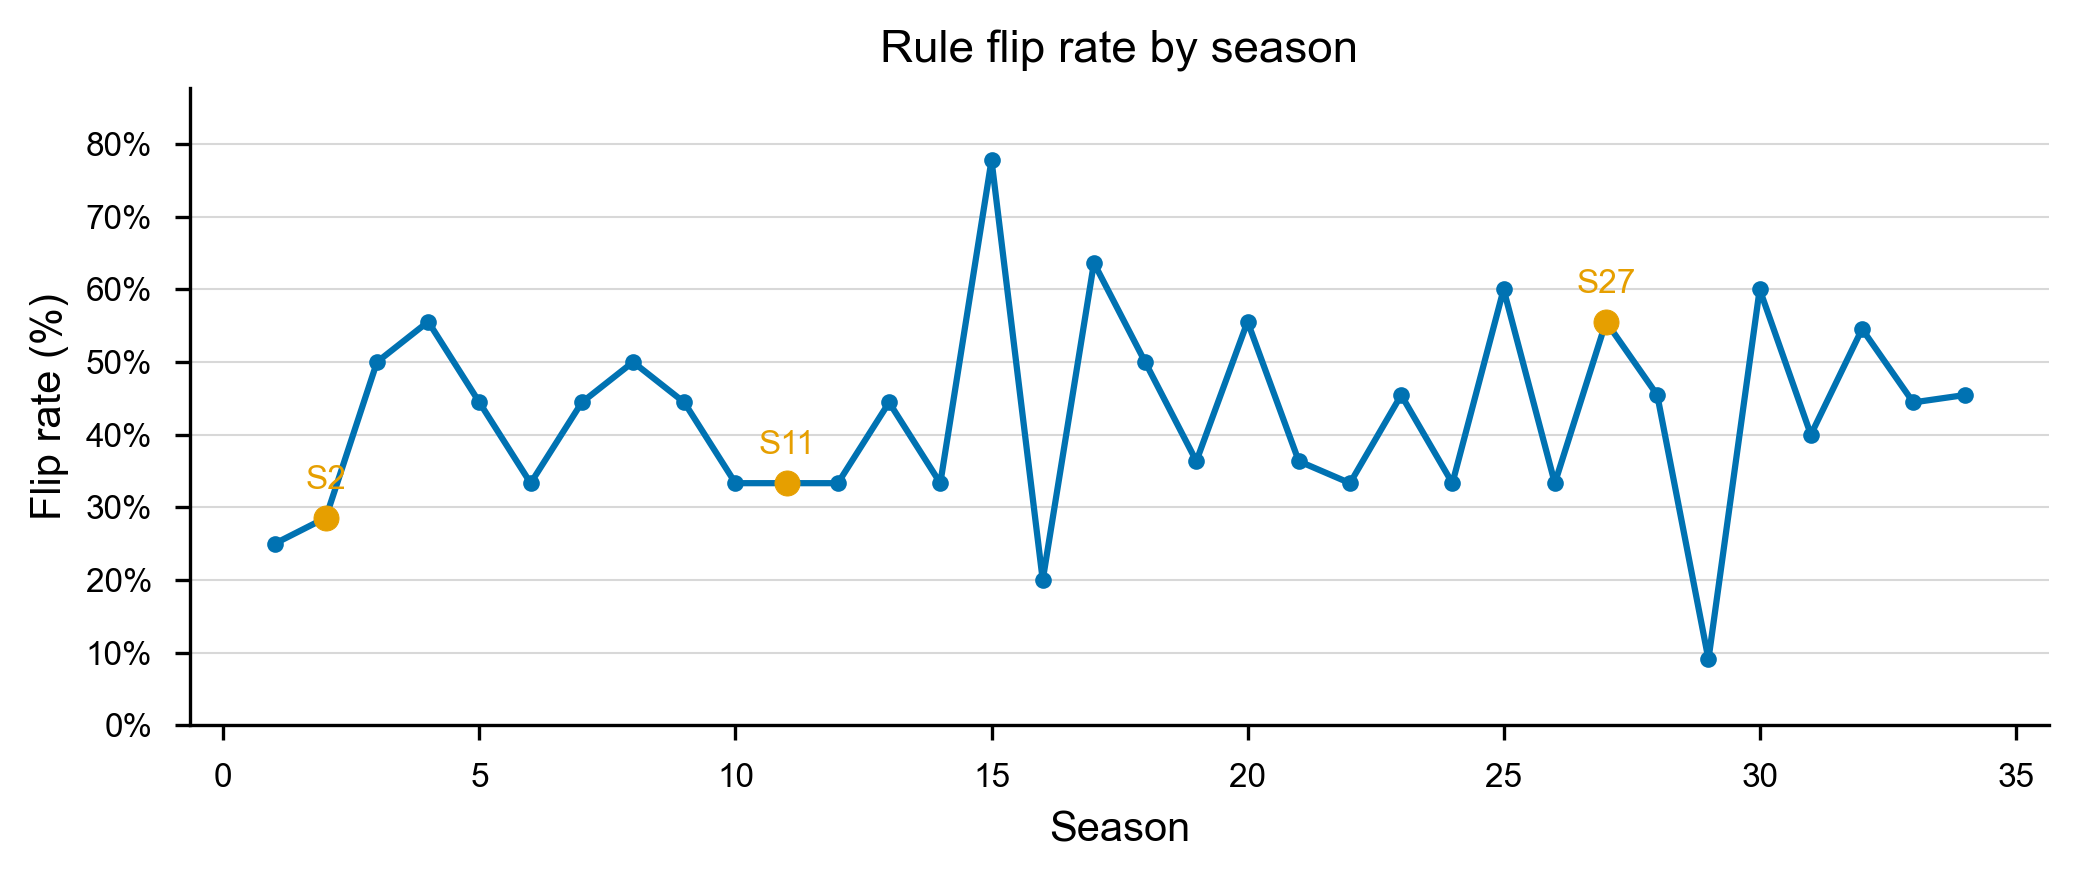
\includegraphics[width=0.68\textwidth]{../../figures/counterfactual/timeseries_flip_rate_by_season_v1.png}
\caption{Flip rate evolution across seasons, revealing temporal patterns of rule sensitivity.}
\label{fig:flip_rate_evolution}
\end{figure}

%===============================================================================
% SECTION 7: PROBLEM 3 - DETERMINANTS OF SUCCESS
%===============================================================================
% SECTION 7: PROBLEM 3 - DETERMINANTS OF SUCCESS
%===============================================================================

\section{Problem 3: Determinants of Success}
After comparing how different voting rules alter outcomes, we now examine which factors determine success and how judges and fans weigh these factors.
We treat the proxy metric Mfan for fan votes and Mjudge for judge scores as outcome variables, analyzing four feature groups:
Time features include weeks to capture the impact of specific phases on engagement and performance.
Performance characteristics encompass relative judge scores and cumulative average scores, summarizing contestants' rankings and consistency.
Demographic characteristics cover star age and industry affiliation, reflecting learning ability, stage presence, fan base diversity, and public recognition.
Partner characteristics include professional dancers' average ranking, experience level, and win rate, collectively reflecting
the dancer's contribution to the star's competition results.
\begin{figure}[H]
\centering
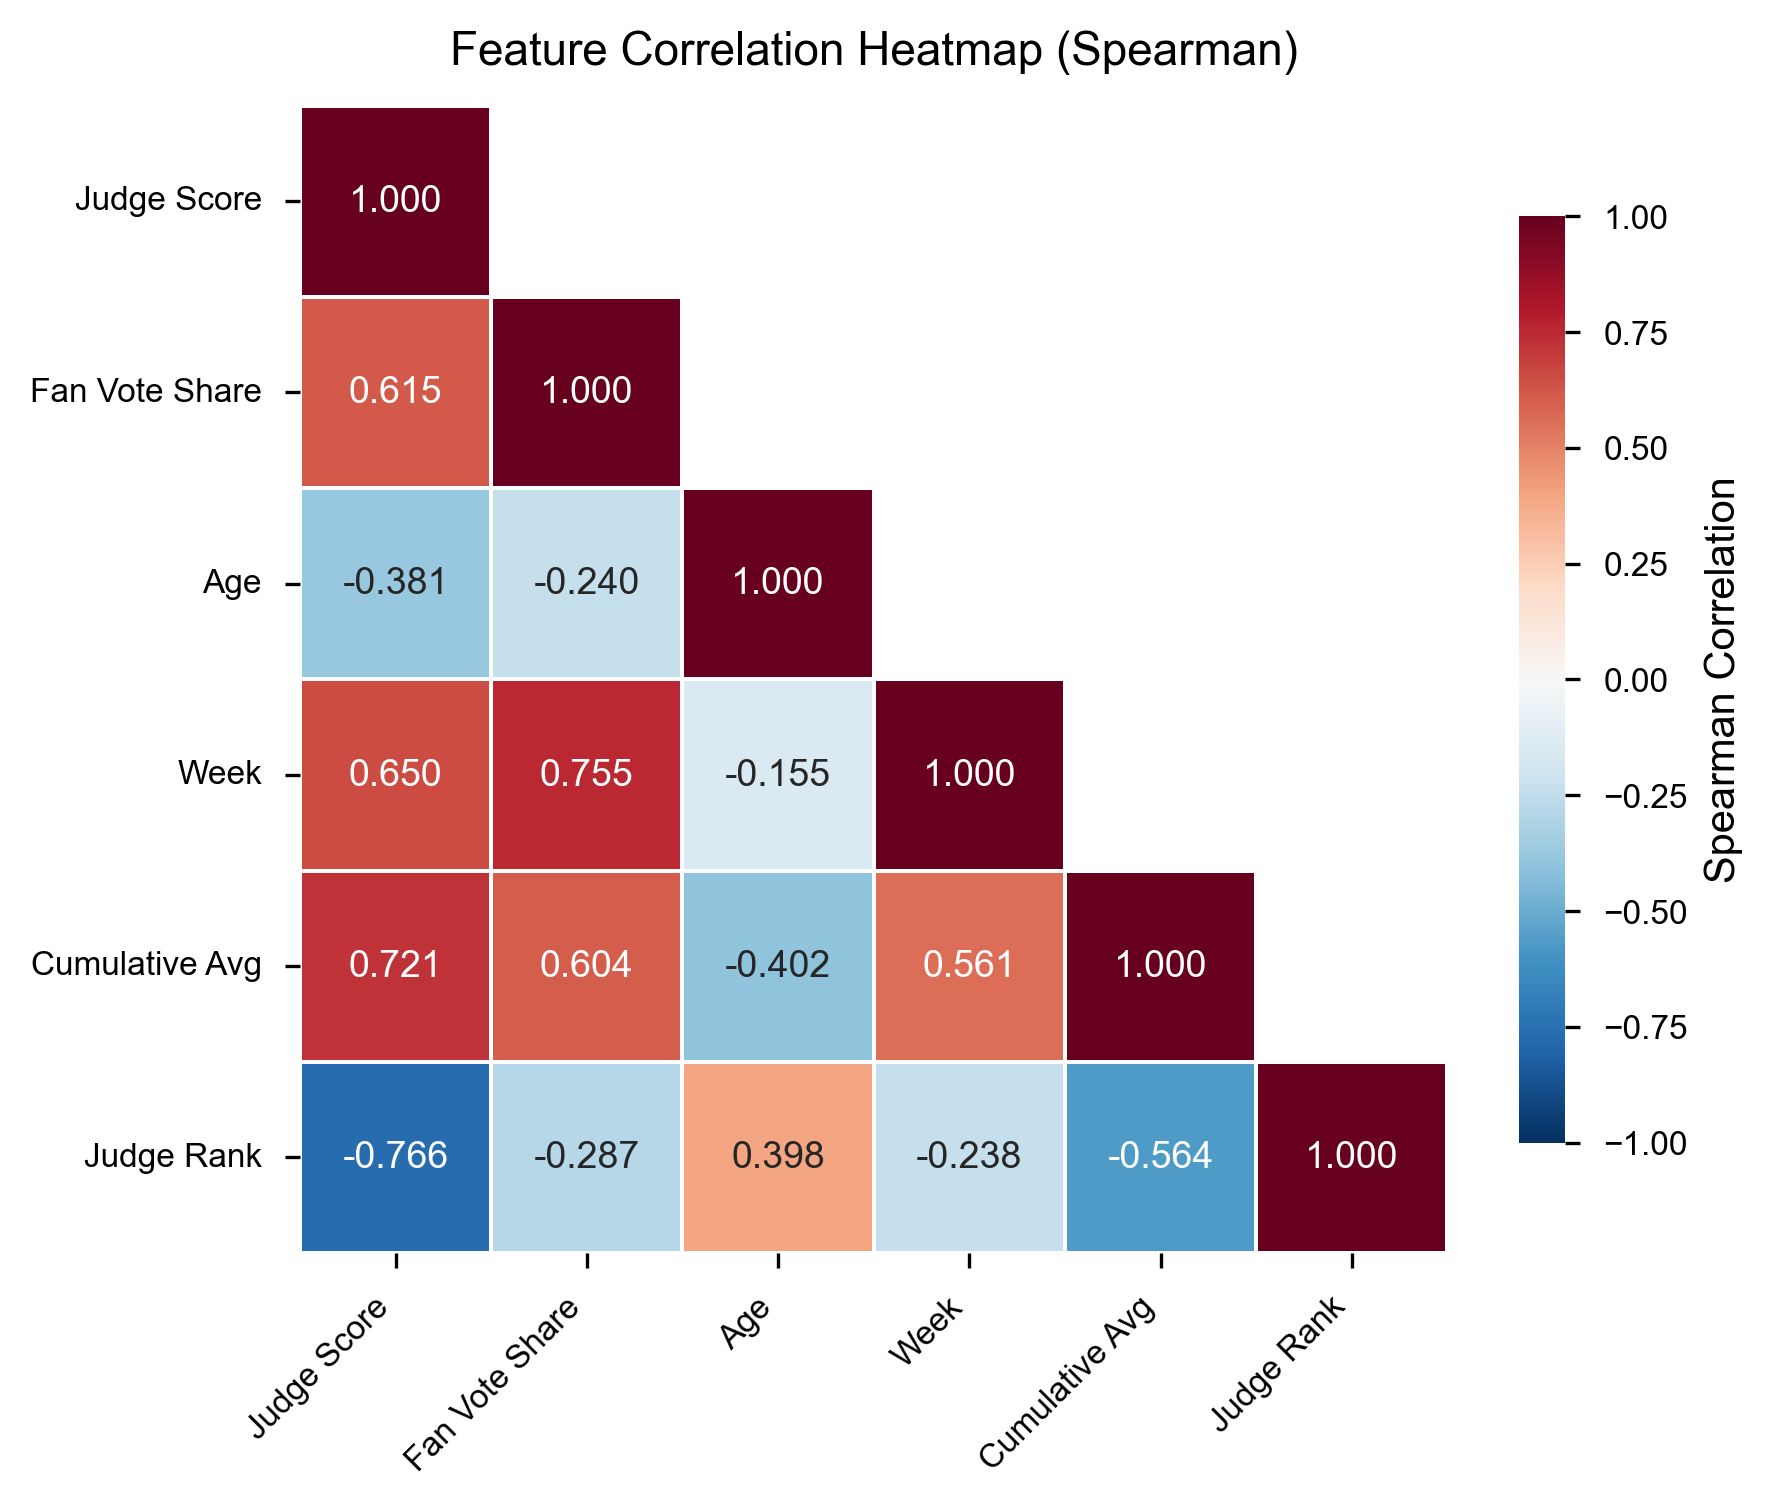
\includegraphics[width=0.60\textwidth]{../../figures/twin_model/correlation_heatmap.png}
\caption{Spearman correlation heatmap}
\label{fig:correlation_heatmap}
\end{figure}

\subsection{Twin Random Forest Model construction}
To address our core research objective—analyzing the discrepancies between judge scores and
fan votes, and elucidating their differential mechanisms across various features—we innovatively
employ a Twin Random Forest (TRF) architecture. This framework constructs two independent
random forest\cite{2} models to predict contestant performance based on fan votes (Mfan) and judge scores
(Mjudge) respectively. Compared to single-model or conventional machine learning approaches
, this dual-model architecture is tailored to our research
needs. Both independent models aim to predict contestant outcomes 
with a unified mathematical formulation ensuring logical consistency and normative rigor
\vspace{-0.5em}
\begin{figure}[H]
  \centering
  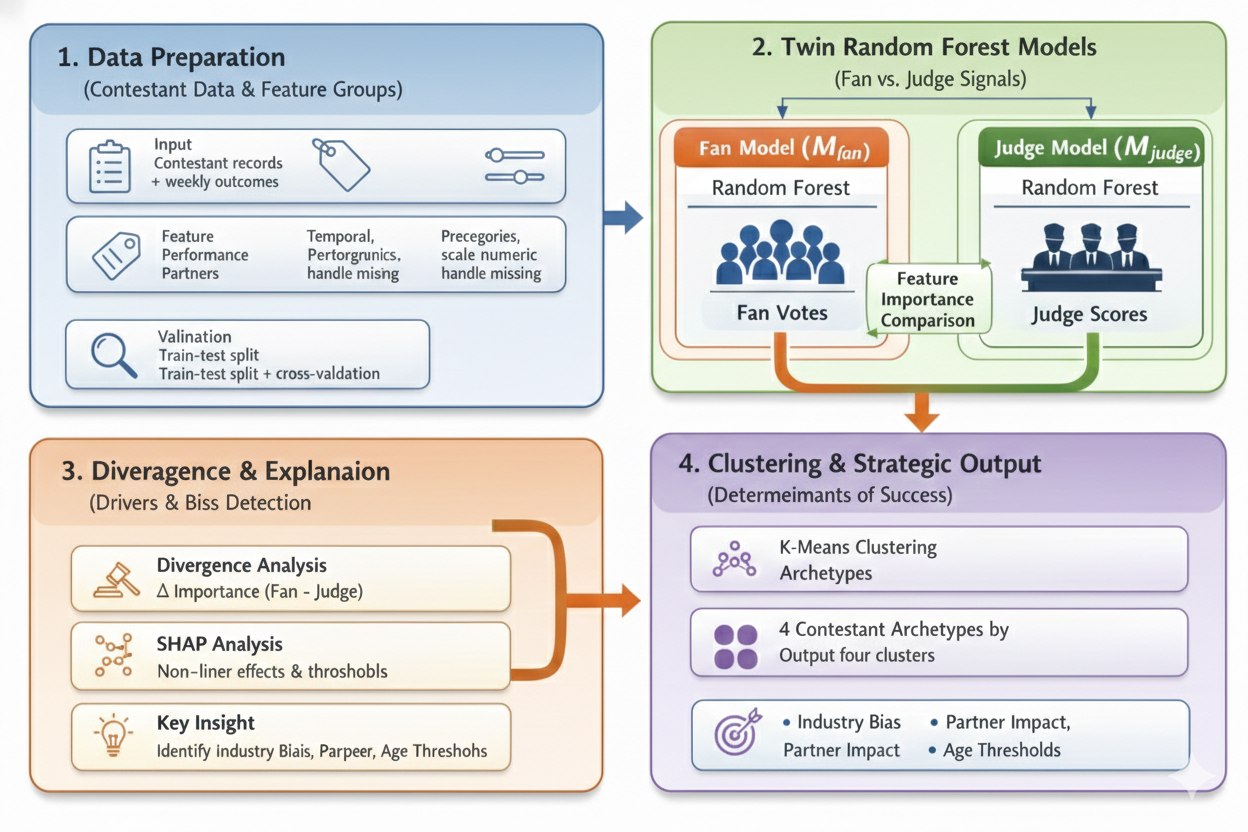
\includegraphics[width=0.6\textwidth]{../../Draw_picture/Gemini_Generated_Image_88h8u988h8u988h8.png}
  \caption{Twin Random Forest architecture}
  \label{fig:twin_rf_arch}
  \end{figure}

\subsection{Feature Importance and TBC}
\begin{table}[h]
\centering
\caption{Industry bias: Fan vs.\ Judge preferences}
\begin{tabular}{l c c c c}
\toprule
Industry & $n$ & Fan Preference & Judge Preference & Net Bias \\
\midrule
Reality TV Star & 15 & +15.2\% & $-$8.1\% & +23.3\% (Fan Favorite) \\
Athlete & 95 & +8.7\% & $-$3.2\% & +11.9\% (Fan Favorite) \\
Singer/Rapper & 61 & +4.1\% & +2.3\% & +1.8\% (Neutral) \\
Actor/Actress & 128 & $-$6.3\% & +12.4\% & $-$18.7\% (Judge Favorite) \\
\bottomrule
\end{tabular}
\end{table}
\textbf{Technical Bias Coefficient.} We define TBC as the normalized difference in importance assigned to technical performance:
\begin{equation}
TBC = \frac{I^{\text{judge}}_{\text{score}} - I^{\text{fan}}_{\text{score}}}{I^{\text{judge}}_{\text{score}} + I^{\text{fan}}_{\text{score}}} = \frac{0.846 - 0.197}{0.846 + 0.197} = 0.612
\end{equation}

\textbf{Interpretation.} TBC = 0.612 indicates judges weight technical performance \textbf{61.2\% more} than fans. Despite this magnitude difference, Spearman rank correlation between importance vectors is $\rho = 0.929$ ($p = 0.0025$)---both groups recognize the same factors as important but disagree on how much each matters.

\subsection{SHAP Analysis: Nonlinear Effects}

Global feature importance does not reveal nonlinear or instance-level effects. We therefore use SHAP\cite{3}, Shapley Additive Explanations, to attribute each prediction to individual features. SHAP provides individualized explanations by decomposing each prediction into additive feature contributions based on cooperative game theory. 

The contribution of feature $x_i$ for a given observation is defined by the Shapley value over the model $f$:
\begin{equation}\label{eq:shap_single}
\text{SHAP}_i = \sum_{S \subseteq X \setminus \{x_i\}} \frac{|S|! (k - |S| - 1)!}{k!} \left[ f(S \cup \{x_i\}) - f(S) \right]
\end{equation}
Here $S$ runs over all subsets of features excluding $x_i$, $X$ is the full feature set, $k$ is the number of features, and the weight $\frac{|S|! (k - |S| - 1)!}{k!}$ is the usual Shapley kernel\cite{4} ensuring fair attribution. The term $f(S \cup \{x_i\}) - f(S)$ measures the marginal contribution of adding feature $x_i$ to coalition $S$. A positive $\text{SHAP}_i$ means that feature $i$ raises the predicted outcome; a negative value means it lowers it.

We compute SHAP values for both the fan and judge Twin Random Forest models, aggregating over all contestant-week observations to identify systematic patterns. This yields a local, additive explanation for each contestant-week and allows comparison of nonlinear effects across features, including threshold effects and interaction patterns. The resulting SHAP distributions support both instance-level interpretation and population-level contrast between judge and fan preference structures.

\begin{figure}[H]
\centering
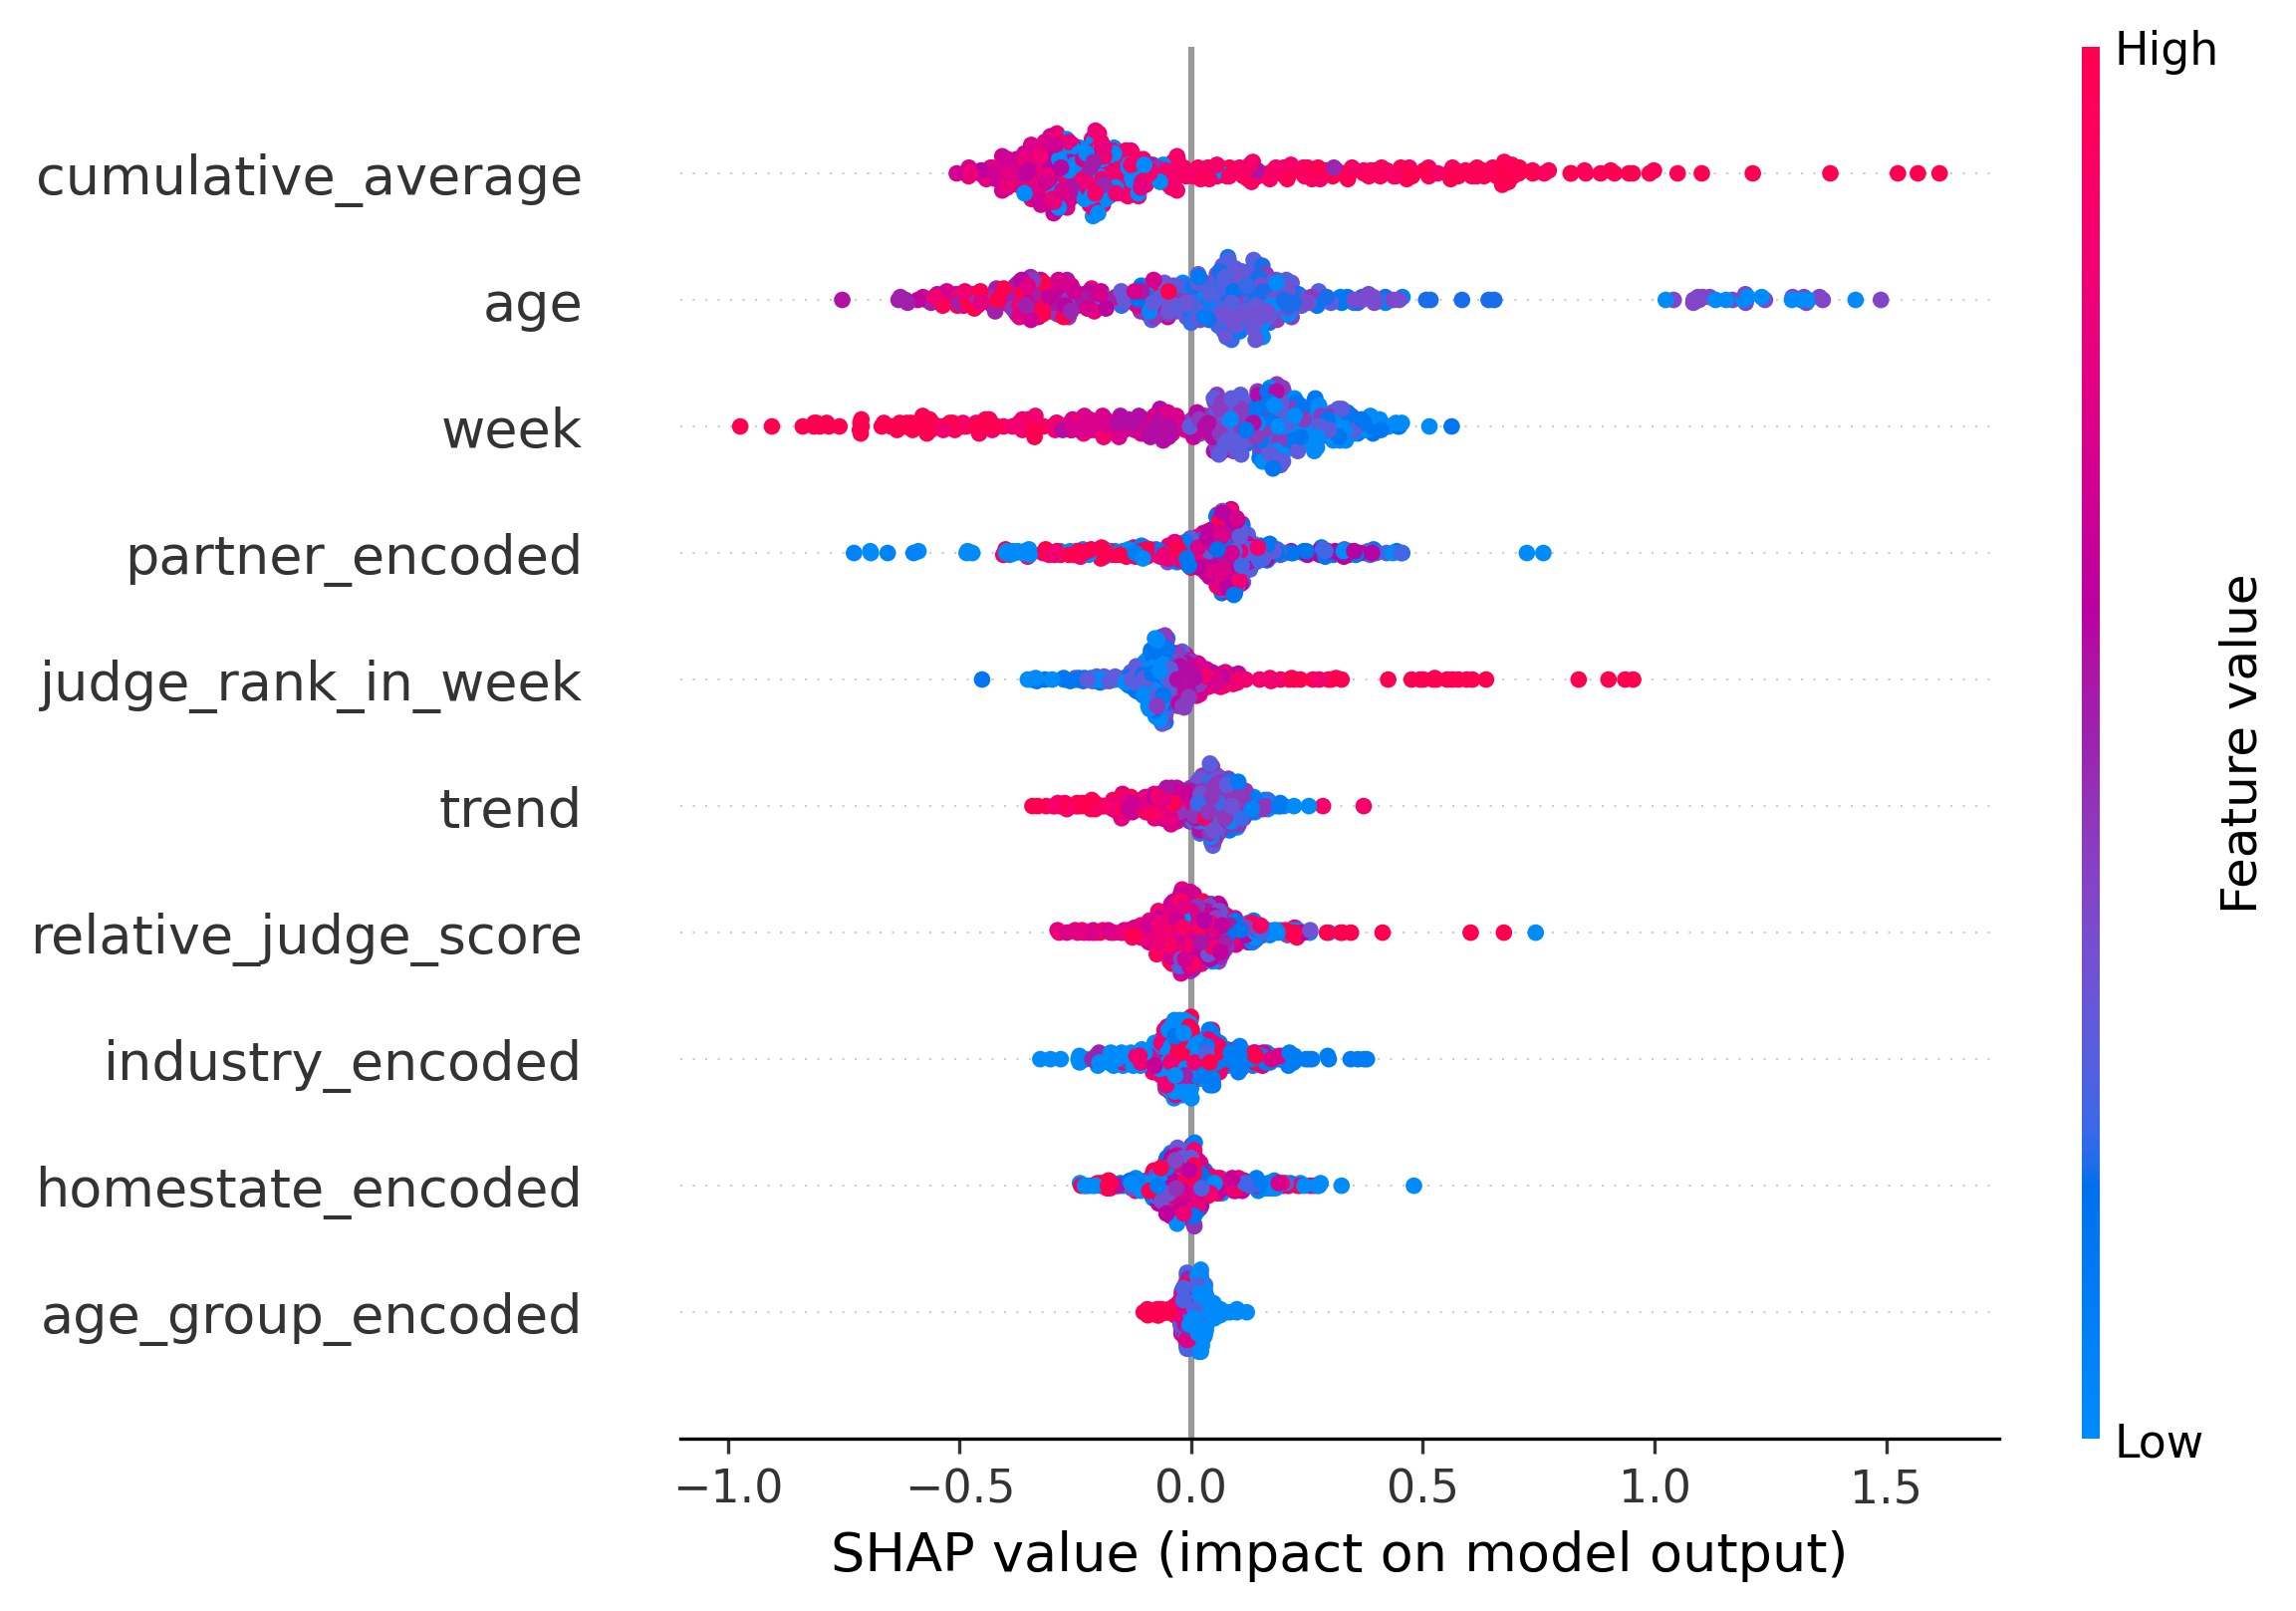
\includegraphics[width=0.68\textwidth]{../../figures/shap_analysis/shap_summary_plot.png}
\caption{SHAP summary plot}
\end{figure}

Taking the age of celebrities as an example, its nonlinear impact on fan support can be quantified by the mean SHAP values of different age groups, with the specific calculation formula as follows:
\begin{equation}\label{eq:shap_age}
SHAP_{age} = \sum_{i=1}^{n} \frac{1}{n} \left[ \frac{I_{age<40}}{I_{age>40}} \right] \cdot SHAP_{age,i}
\end{equation}
where $SHAP_{age,i}$ is the SHAP value of the age feature in the $i$-th observation, and $I_{age<40}$, $I_{age>40}$ are indicator functions (taking a value of 1 if the corresponding condition is satisfied, and 0 otherwise). Through empirical calculations, we find that the mean SHAP value of players under 40 years old is +0.17 (exerting a positive contribution to fan votes), and the mean SHAP value of players over 40 years old is -0.33 (exerting a negative contribution to fan votes). This result clearly identifies the 40-year-old threshold effect of age on fan support, which provides an important empirical support for the subsequent summary of research conclusions.

\begin{figure}[H]
\centering
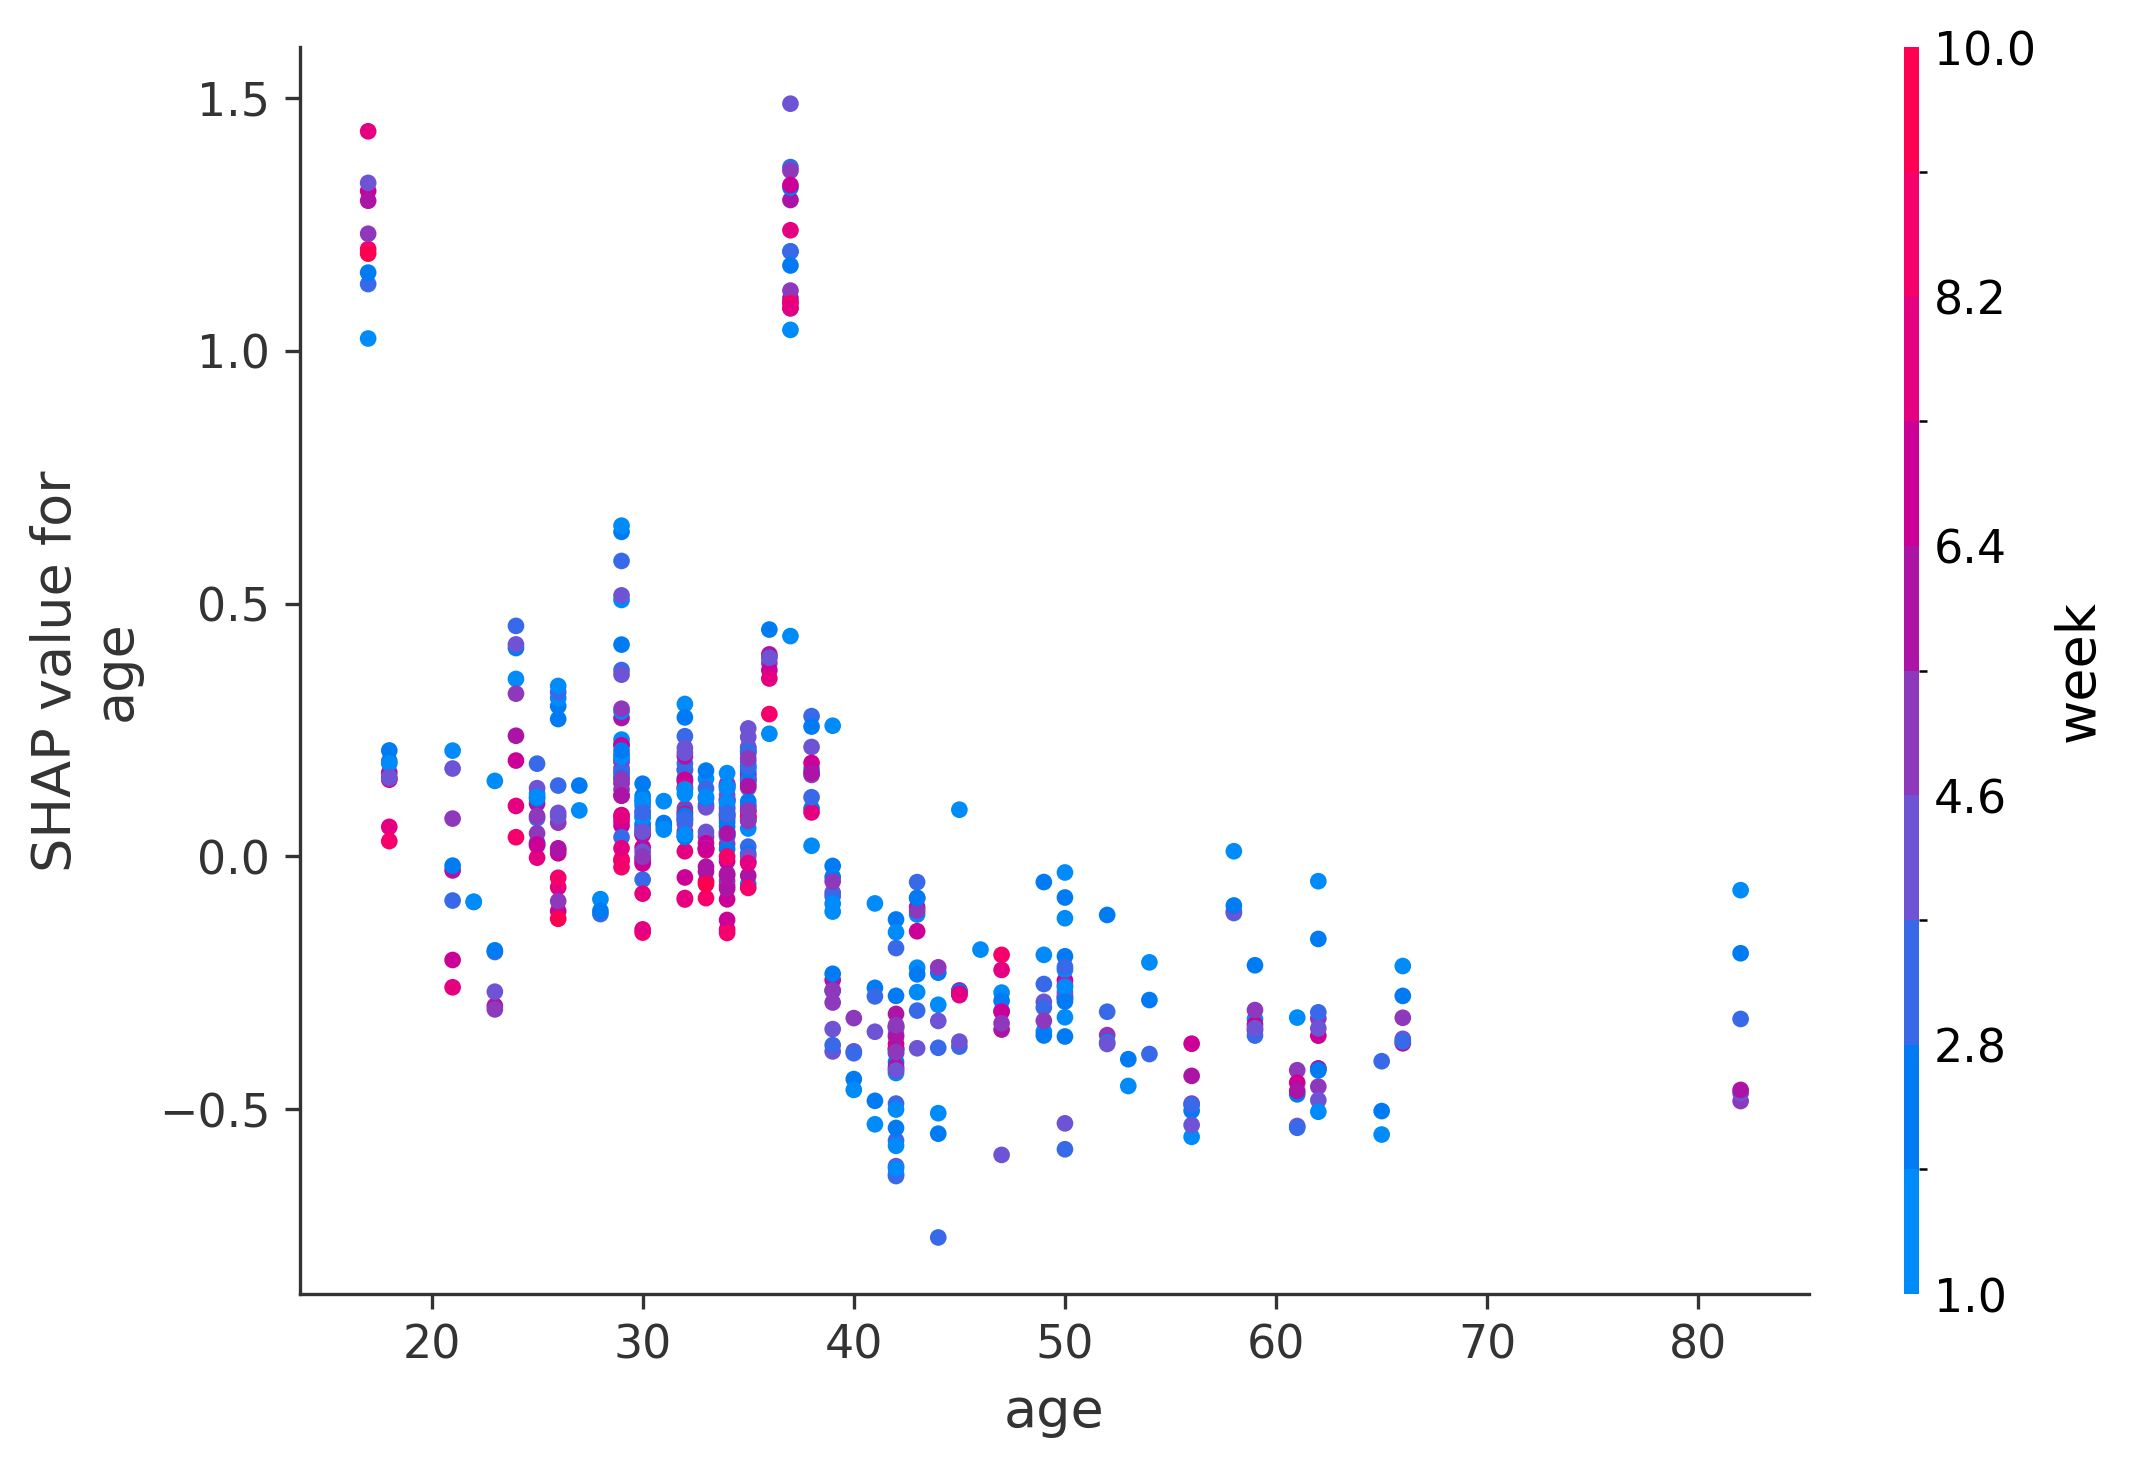
\includegraphics[width=0.48\textwidth]{../../figures/shap_analysis/shap_dependence_age.png}
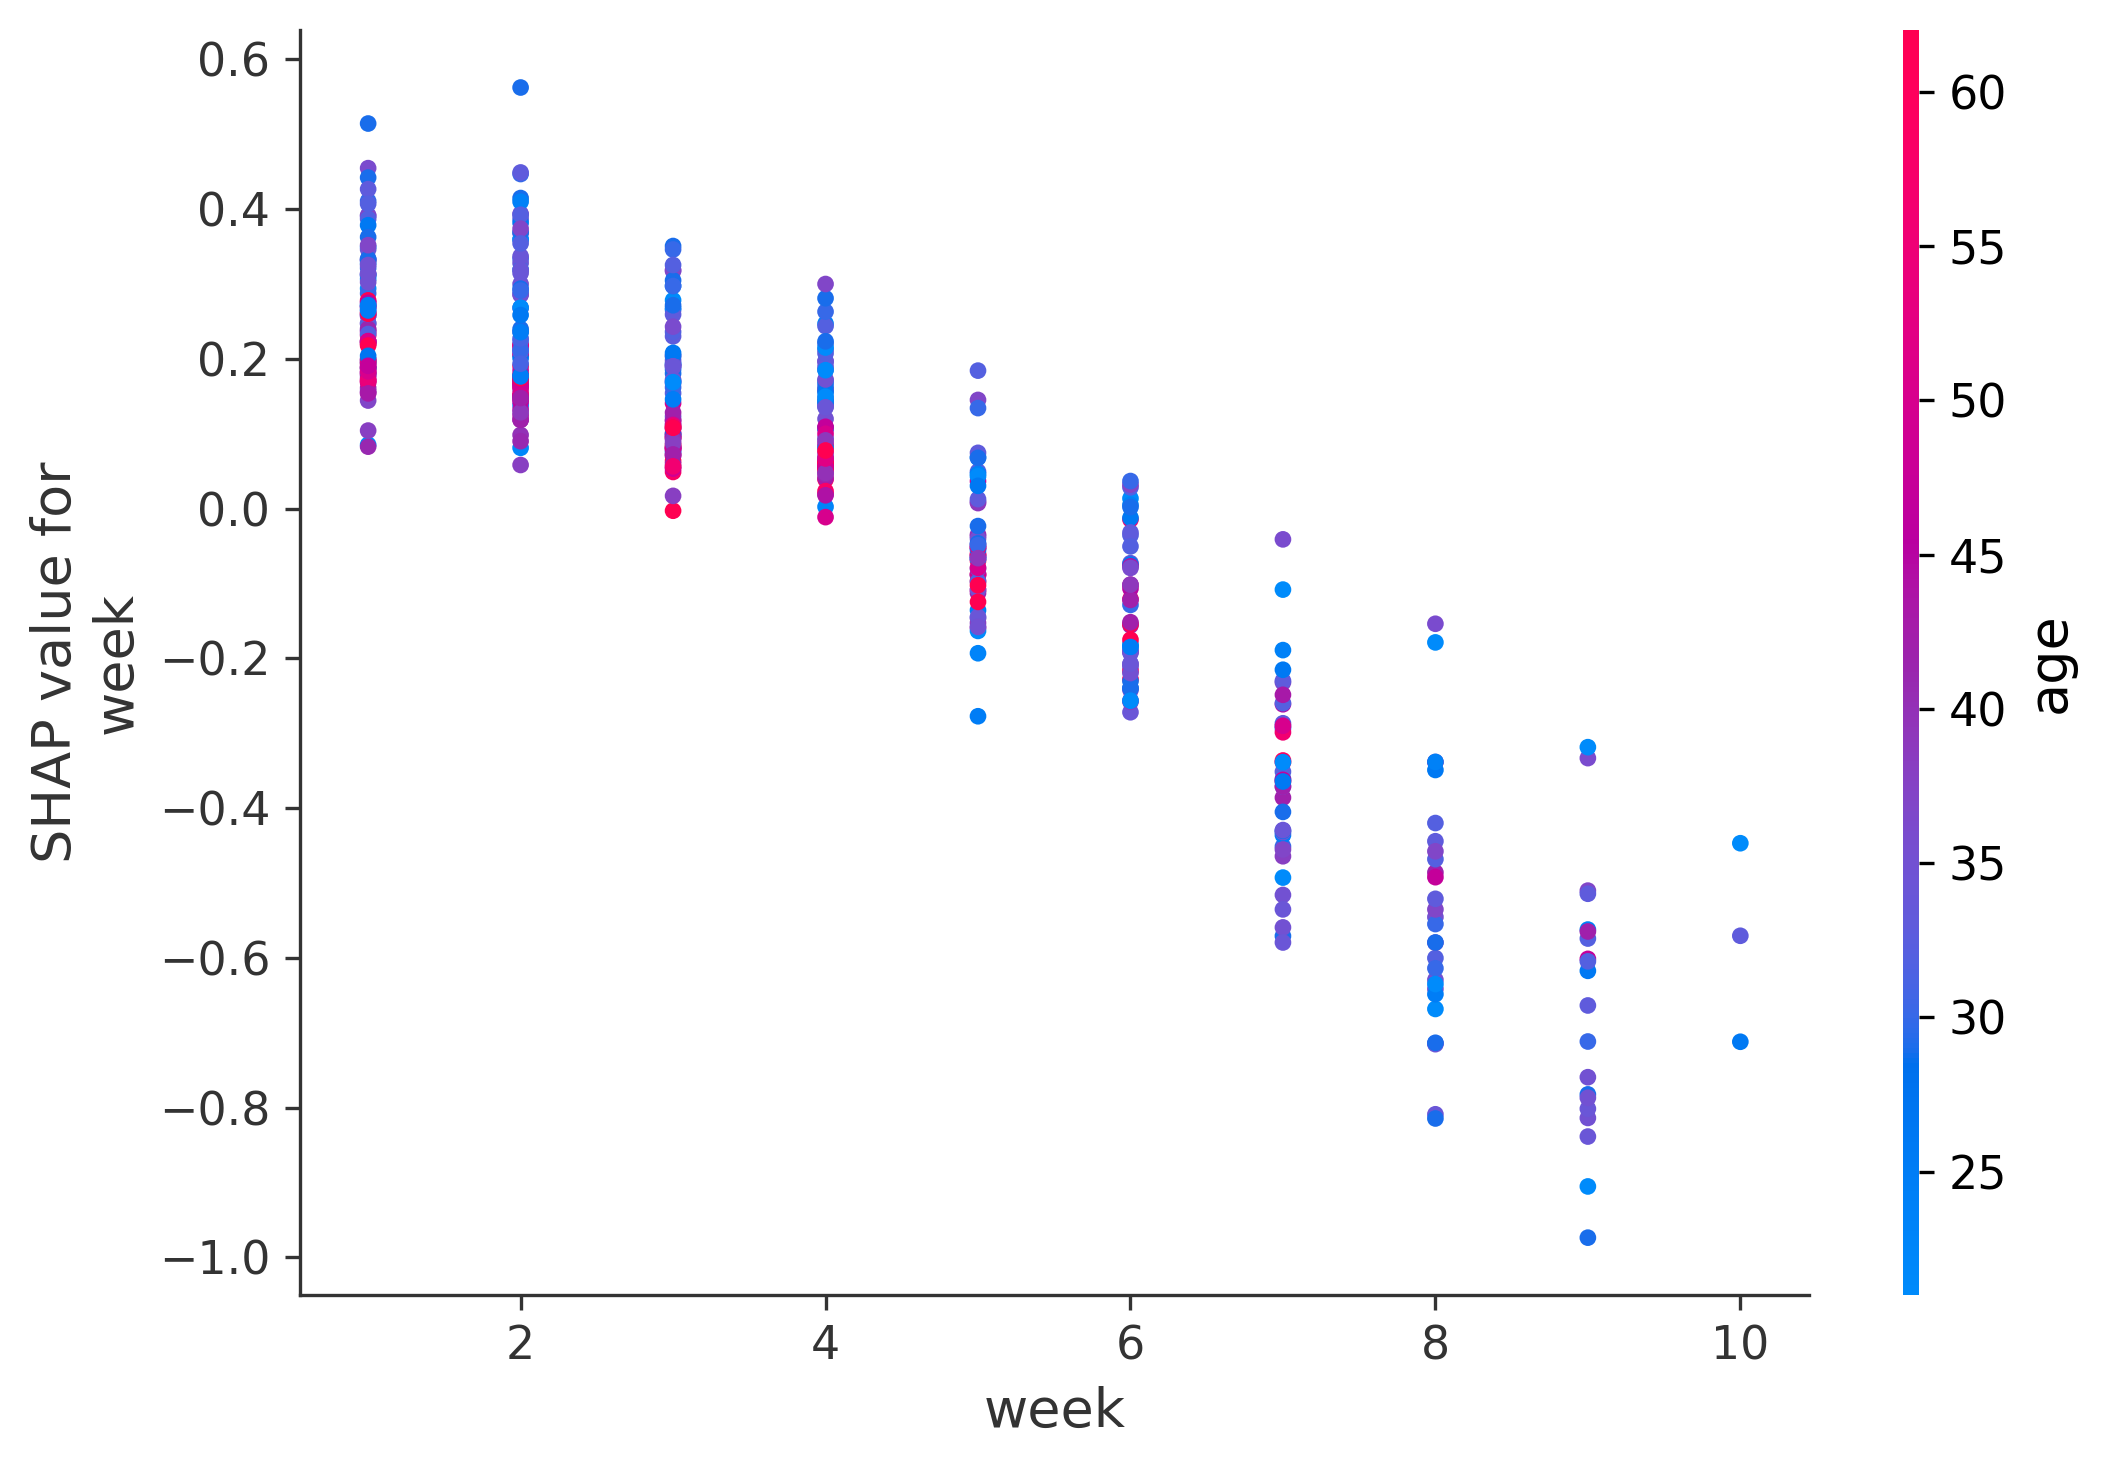
\includegraphics[width=0.48\textwidth]{../../figures/shap_analysis/shap_dependence_week.png}
\caption{SHAP age 40 threshold  \& week importance for fan loyalty}
\end{figure}

SHAP yields three main nonlinear effects. Age exhibits a threshold near 40: mean SHAP is about $+0.17$ for contestants under 40 and about $-0.33$ for those 40 or older, so younger contestants receive higher fan support on average. Partner quality carries strongly---SHAP contributions span roughly $-0.73$ to $0.76$, and stronger partners are associated with about 2.3 fewer placement ranks, with correlation $\rho \approx -0.31$. Temporal dynamics differ by stakeholder: week accounts for about 64\% of importance in the fan model but only about 7\% in the judge model, consistent with fans rewarding loyalty over time.

\subsection{Industry Bias Analysis}
Industry affects fan and judge evaluations differently because of differences in fan base, visibility, and stage style. We define net bias as $\text{Net\_Bias} = I_{\text{fan}} - I_{\text{judge}}$, where $I_{\text{fan}}$ and $I_{\text{judge}}$ are normalized industry importance in the fan and judge models in $[0,1]$. Net bias lies in $[-1,1]$; positive values indicate fan-preferred industries and negative values indicate judge-preferred ones. Empirically, Reality TV stars show net bias about $+23.3\%$ and actors about $-18.7\%$, a 42\% swing---consistent with stronger fan bases for reality TV and stronger alignment with technical criteria for actors. Figure~\ref{fig:industry_bias} summarizes these patterns.
\begin{figure}[H]
\centering
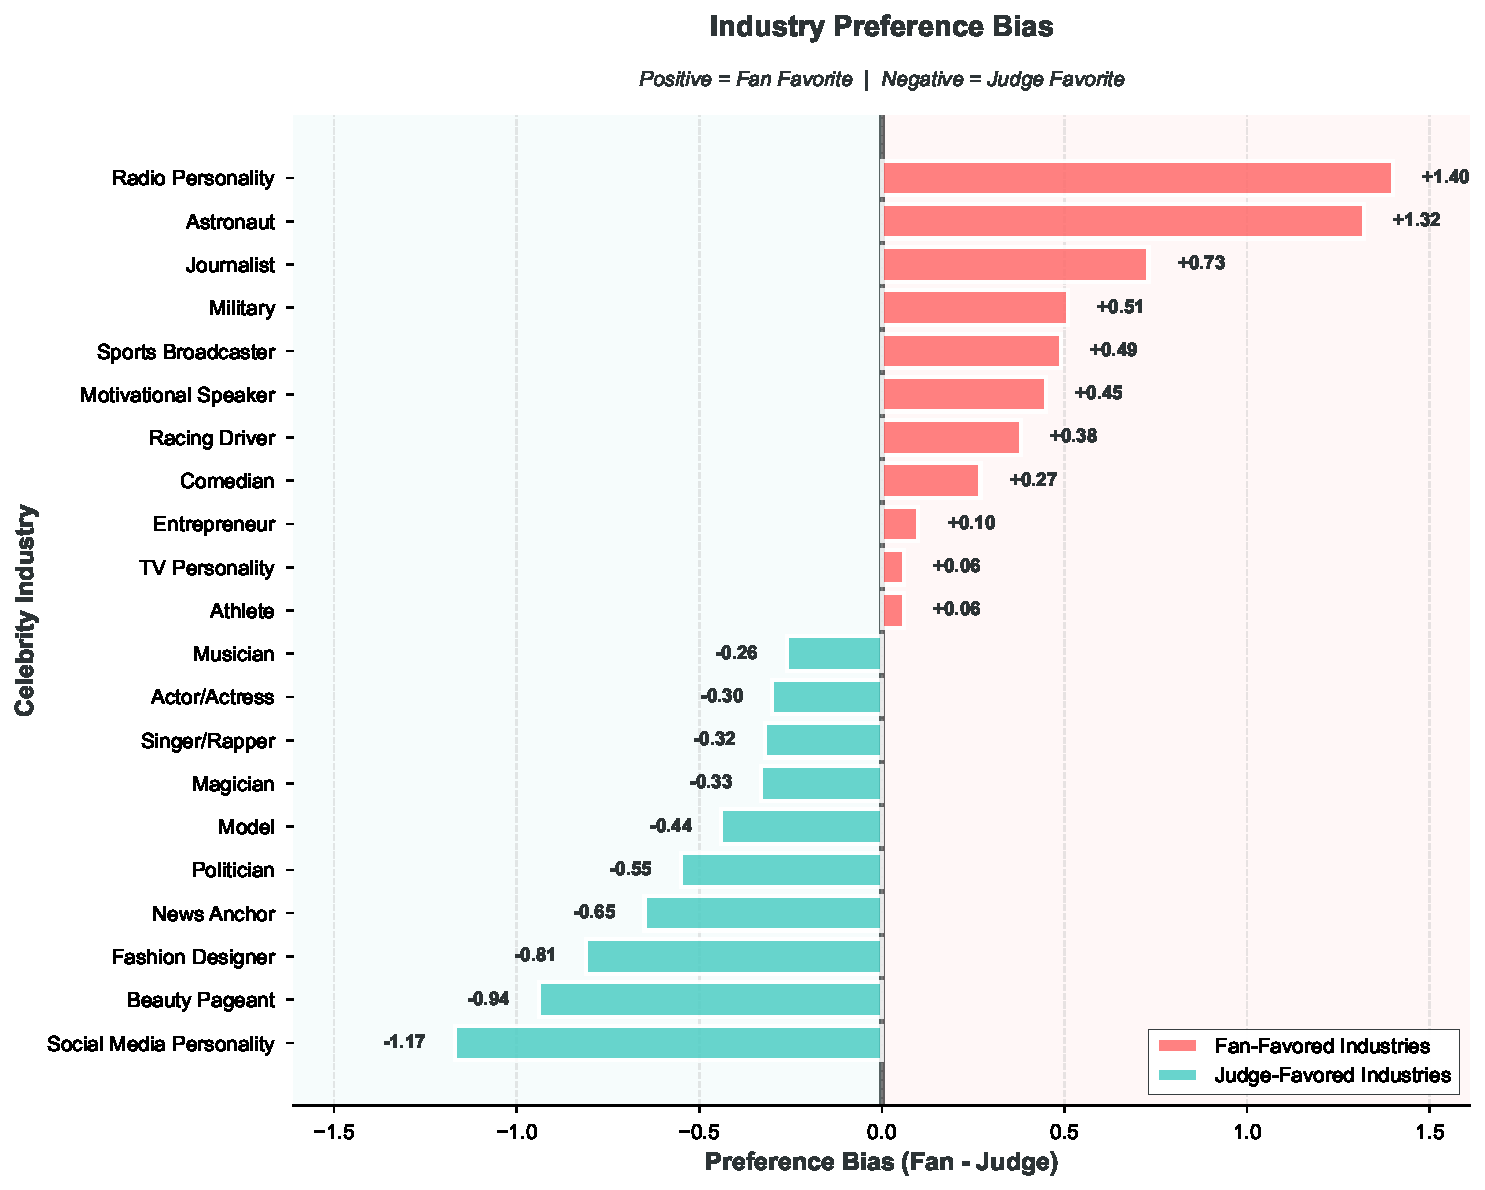
\includegraphics[width=0.65\textwidth]{../../figures/twin_model/industry_bias_improved.pdf}
\caption{Industry bias comparison}
\label{fig:industry_bias}
\end{figure}

%%Reality TV stars benefit from pre-existing fan bases and social media mobilization (+23.3\% net fan bias), while actors benefit from theatrical expression ($-$18.7\% net judge bias). This 42\% swing demonstrates systematic industry effects.


\subsection{Contestant Archetypes}
We cluster contestants in the plane of normalized judge score $M_{\text{judge}}'$ and fan-vote proxy $M_{\text{fan}}'$ using K-means with $k=4$ chosen by the elbow method. Centers and assignments are updated by minimizing the sum of squared Euclidean distances:
\begin{equation}
\text{SSE} = \sum_{j=1}^4 \sum_{z \in S_j} \| z - c_j \|^2,
\end{equation}
where $S_j$ is the $j$-th cluster and $c_j$ its center. We use K-means++ initialization and stop at convergence; Silhouette coefficient is 0.72. The four archetypes: 
\\\hspace*{1em}\textbf{Superstars} (39\%, high--high): average placement 3.0 with consistently strong judge scores and fan support, indicating dominant all-around performers. 
\\\hspace*{1em}\textbf{Tech Giants} (21\%, high--low): technically strong but relatively weaker fan pull; for example, Sabrina Bryan (S5) was eliminated in Week 6 despite high scores. 
\\\hspace*{1em}\textbf{Fan Favorites} (3.6\%, low--high): a controversy-prone cluster where popularity outweighs technical merit; examples include Bobby Bones (S27), Jerry Rice (S2), and Bristol Palin (S11). 
\\\hspace*{1em}\textbf{Underdogs} (36\%, low--low): average placement 10.1, typically facing pressure from both limited fan support and modest technical scores.

\begin{figure}[H]
  \centering
  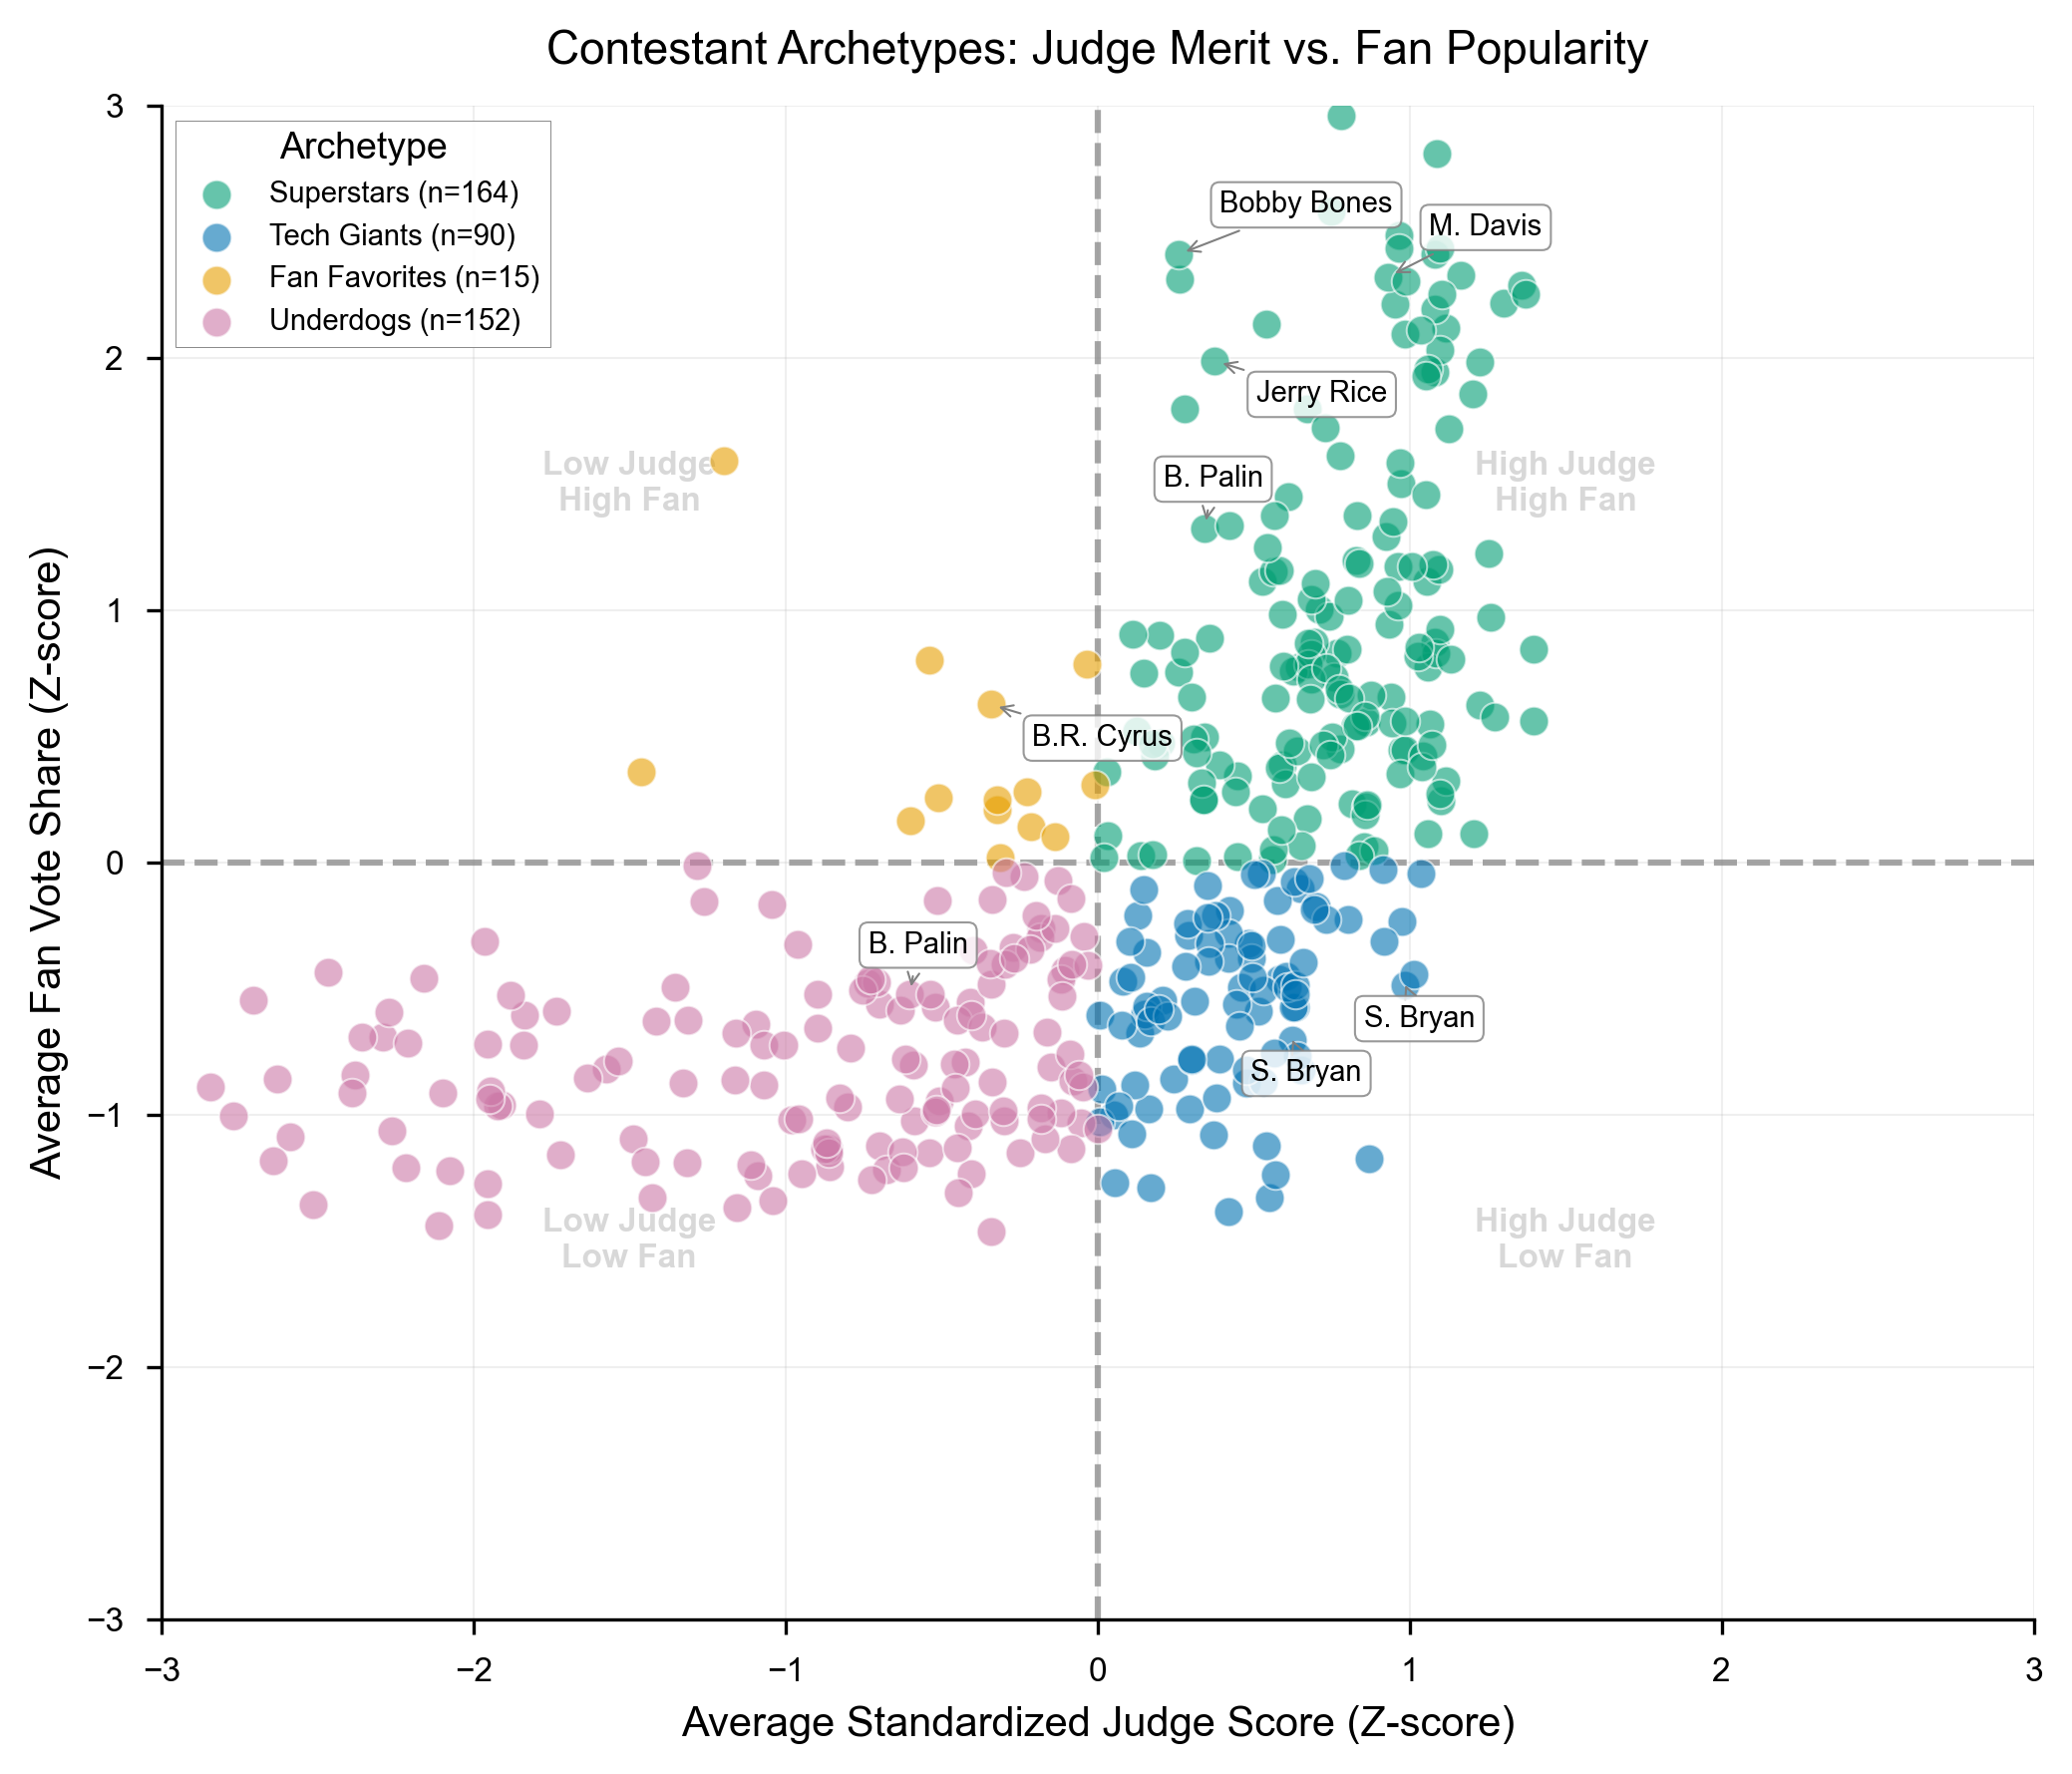
\includegraphics[width=0.6\textwidth]{../../figures/twin_model/contestant_clustering.png}
  \caption{Contestant archetypes}
  \label{fig:contestant_clustering}
  \end{figure}

\subsection{Conclusion}
Success determinants differ by stakeholder. Judges weight technical performance about 61\% more than fans; fans weight week far more than judges, consistent with loyalty over time. Age shows a 40-year threshold; partner quality correlates with placement. Industry net bias spans about 42\% between Reality TV and actors. \textbf{Answer to Q3.} Partner and celebrity attributes jointly shape outcomes, but judges emphasize technical execution while fans emphasize temporal loyalty and demographic appeal.



%===============================================================================
% SECTION 8: PROBLEM 4 - SYSTEM OPTIMIZATION
%===============================================================================

%===============================================================================
% SECTION 8: PROBLEM 4 - SYSTEM OPTIMIZATION
%===============================================================================

\section{Problem 4: System Optimization}
\label{sec:awvs}

We design an Adaptive Weighted Voting System that dynamically adjusts stakeholder influence across competition stages while rewarding demonstrated skill improvement.

\subsection{AWVS Design}

AWVS combines three terms: standardized judge score $Z^{J}_{i,t}$, normalized fan share $Z^{F}_{i,t}$, and a trajectory bonus $Trend_{i,t}$. The combined score for contestant $i$ in week $t$ is
\begin{equation}
S^{\text{AWVS}}_{i,t} = \alpha(t) \cdot Z^{J}_{i,t} + (1-\alpha(t)) \cdot Z^{F}_{i,t} + \beta \cdot Trend_{i,t}.
\end{equation}
The judge weight $\alpha(t)$ increases over the season so that early weeks favor audience engagement and later weeks emphasize technical merit:
\begin{equation}
\alpha(t) = \alpha_{\text{base}} + \gamma \cdot \frac{t}{T_{\max}}.
\end{equation}
The trajectory term rewards improvement over the contestant's own moving average $MA^{J}_{i,t-1}$:
\begin{equation}
Trend_{i,t} = \max\left(0,\, J_{i,t} - MA^{J}_{i,t-1}\right).
\end{equation}
Positive deviations receive a bonus scaled by $\beta$; stagnation or decline adds nothing. Early-season voting thus prioritizes entertainment while the finale rewards technical mastery; the trend bonus separates sustained improvement from flat performance. Table~\ref{tab:awvs_weights} gives representative values of $\alpha(t)$; Figure~\ref{fig:awvs_weights} shows the full progression over the competition timeline.

\begin{table}[H]
\centering
\caption{AWVS temporal weight evolution (representative weeks).}
\label{tab:awvs_weights}
\begin{tabular}{c c c c}
\toprule
Week & $\alpha(t)$ & Judge Weight & Fan Weight \\
\midrule
1 & 0.40 & 40\% & 60\% \\
5 & 0.51 & 51\% & 49\% \\
9 & 0.61 & 61\% & 39\% \\
11 (Finals) & 0.70 & 70\% & 30\% \\
\bottomrule
\end{tabular}
\end{table}

Figure~\ref{fig:awvs_weights} illustrates the continuous shift from fan-dominated to judge-dominated weighting. Grid search on Seasons 1--27 yields $\alpha_{\text{base}}=0.4$, $\gamma=0.3$, $\beta=0.5$, with minimum fan weight 30\% at the finale.

\begin{figure}[H]
\centering
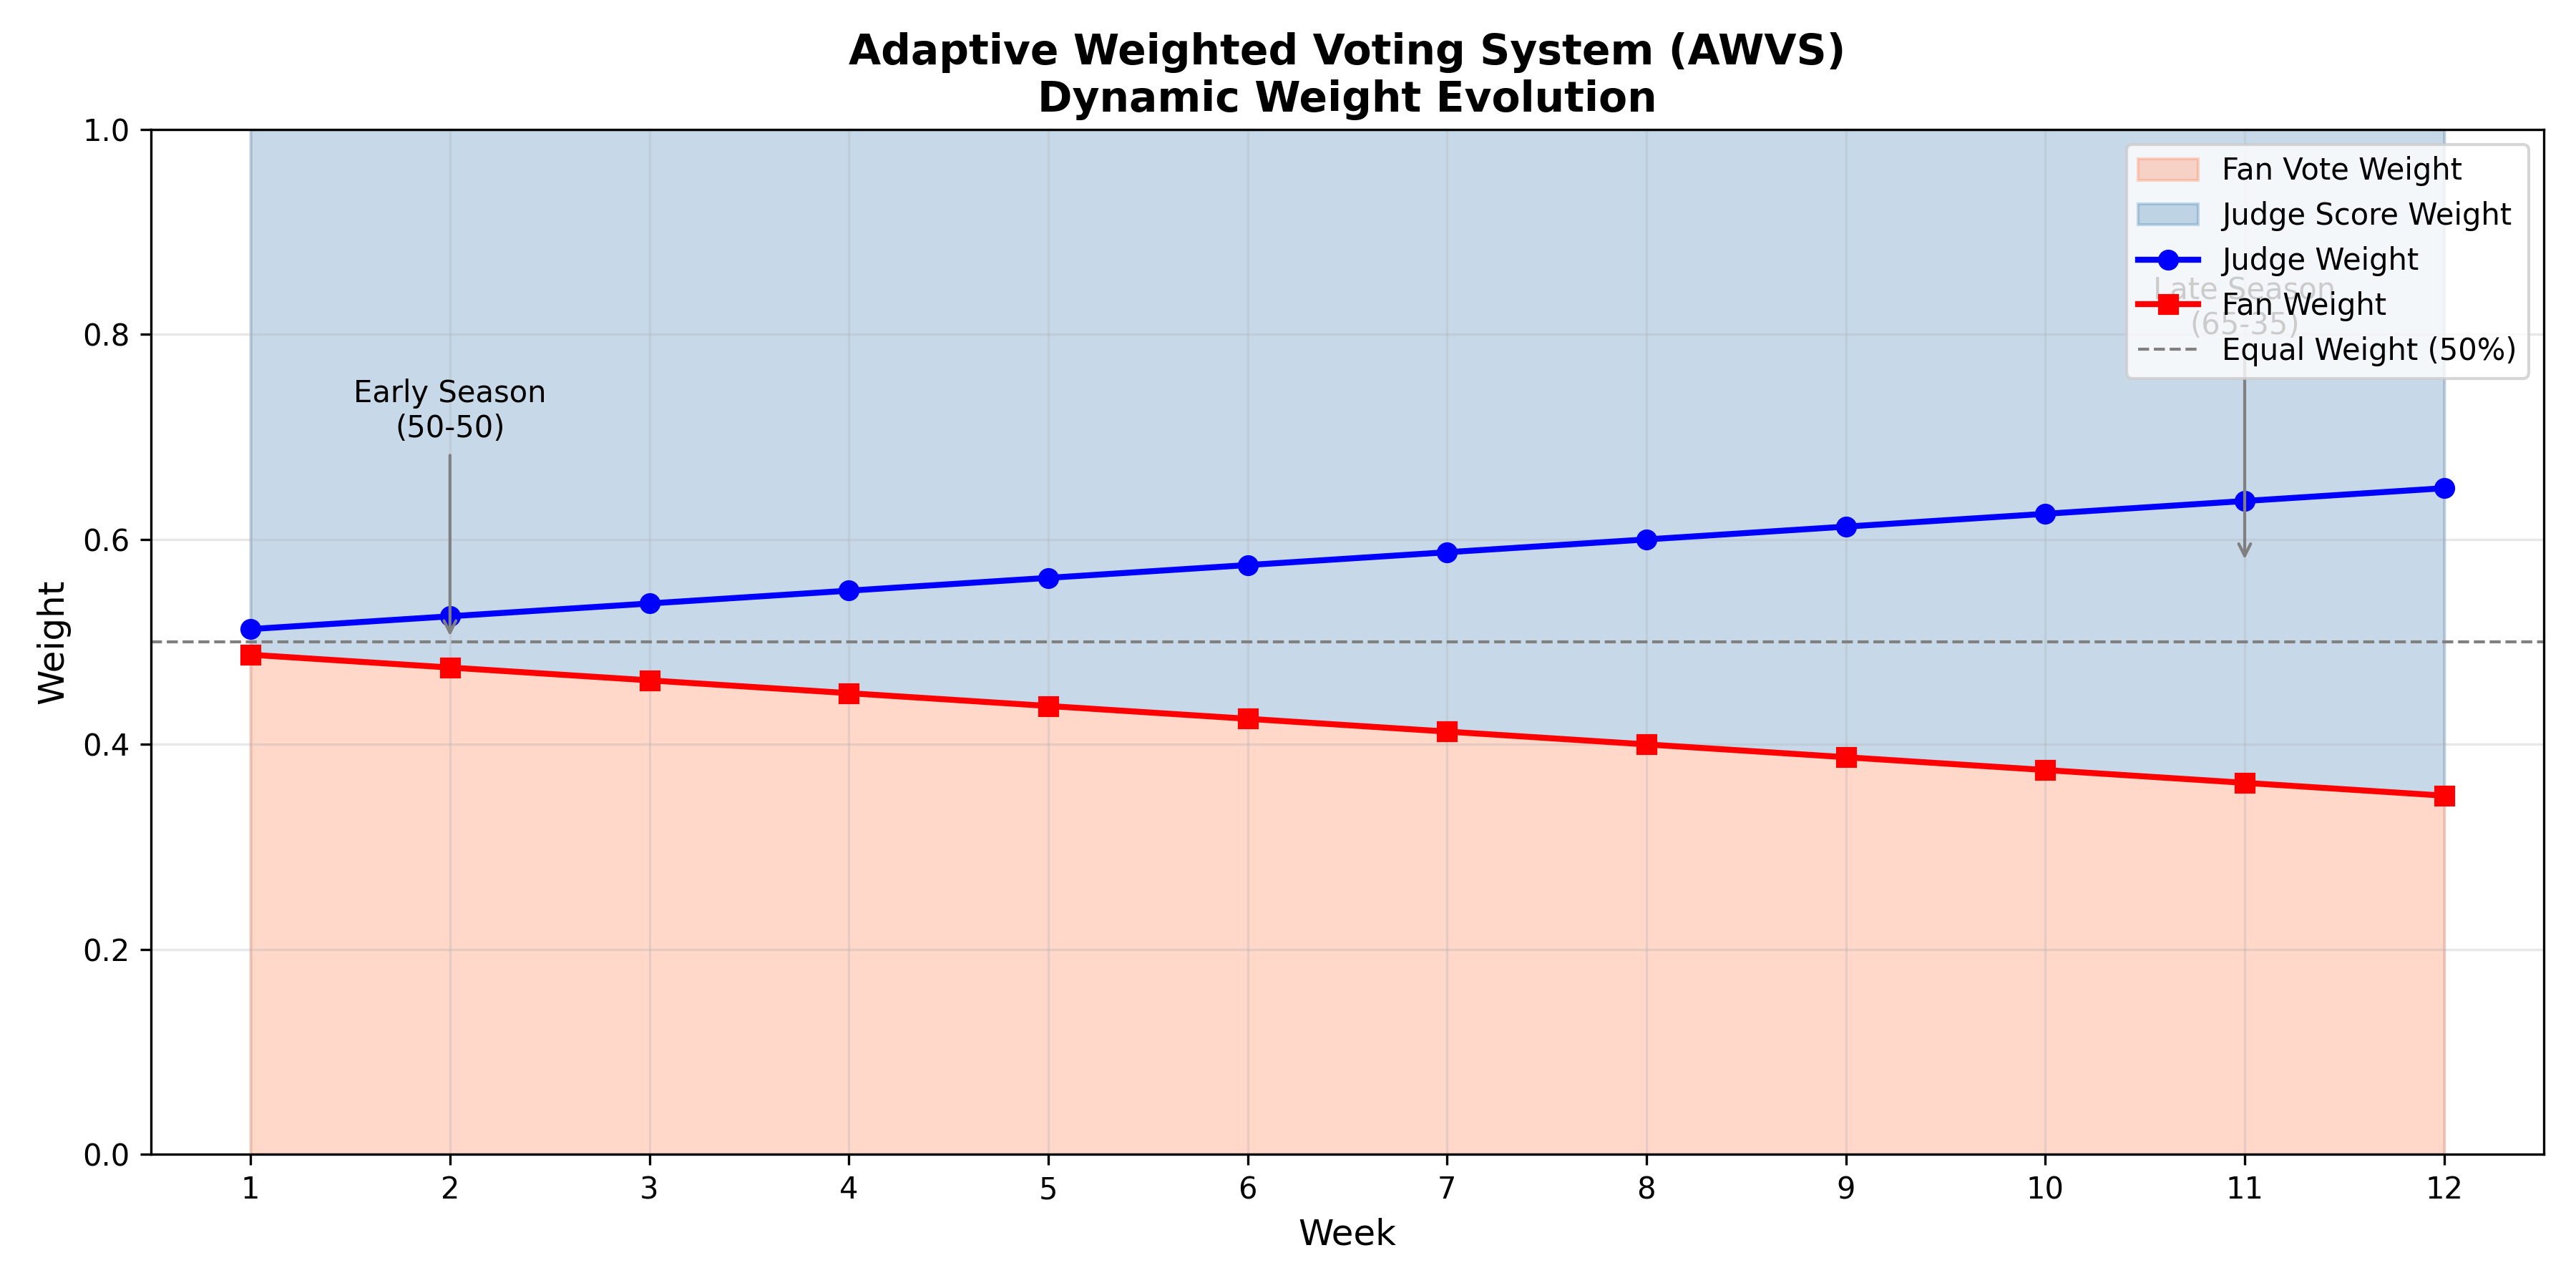
\includegraphics[width=0.78\textwidth]{../../figures/twin_model/weight_evolution.png}
\caption{AWVS judge weight progression over the competition timeline.}
\label{fig:awvs_weights}
\end{figure}

\subsection{Comparative Evaluation}

We conduct retrospective simulation across 241 elimination weeks spanning Seasons 1--27, applying AWVS alongside the three historical rules under identical fan vote estimates. Performance is assessed along four dimensions established in Problem 2: fairness, balance, stability, and technical merit preservation. These metrics are computed identically for all systems to enable direct comparison.

\begin{table}[H]
\centering
\caption{Multi-dimensional performance comparison across voting systems}
\begin{tabular}{l c c c c}
\toprule
Metric & Rank Sum & Percent Sum & Judge Save & \textbf{AWVS} \\
\midrule
Fairness ($1-|\overline{FFI}|$) & 0.866 & 0.813 & 0.759 & \textbf{0.932} \\
Balance (outcome diversity) & 0.913 & 0.772 & 0.589 & \textbf{0.891} \\
Stability ($1-\sigma_{FFI}$) & 0.854 & 0.801 & 0.742 & \textbf{0.889} \\
Technical merit (finals) & 0.810 & 0.850 & 0.730 & \textbf{0.880} \\
\midrule
\textbf{Overall score} & 0.884 & 0.806 & 0.710 & \textbf{0.923} \\
\bottomrule
\end{tabular}
\end{table}

AWVS achieves substantial improvement across all dimensions, with the overall score increasing from 0.884 (Rank Sum) to 0.923, representing enhanced performance in fairness, balance, stability, and technical merit simultaneously.

\begin{figure}[H]
\centering
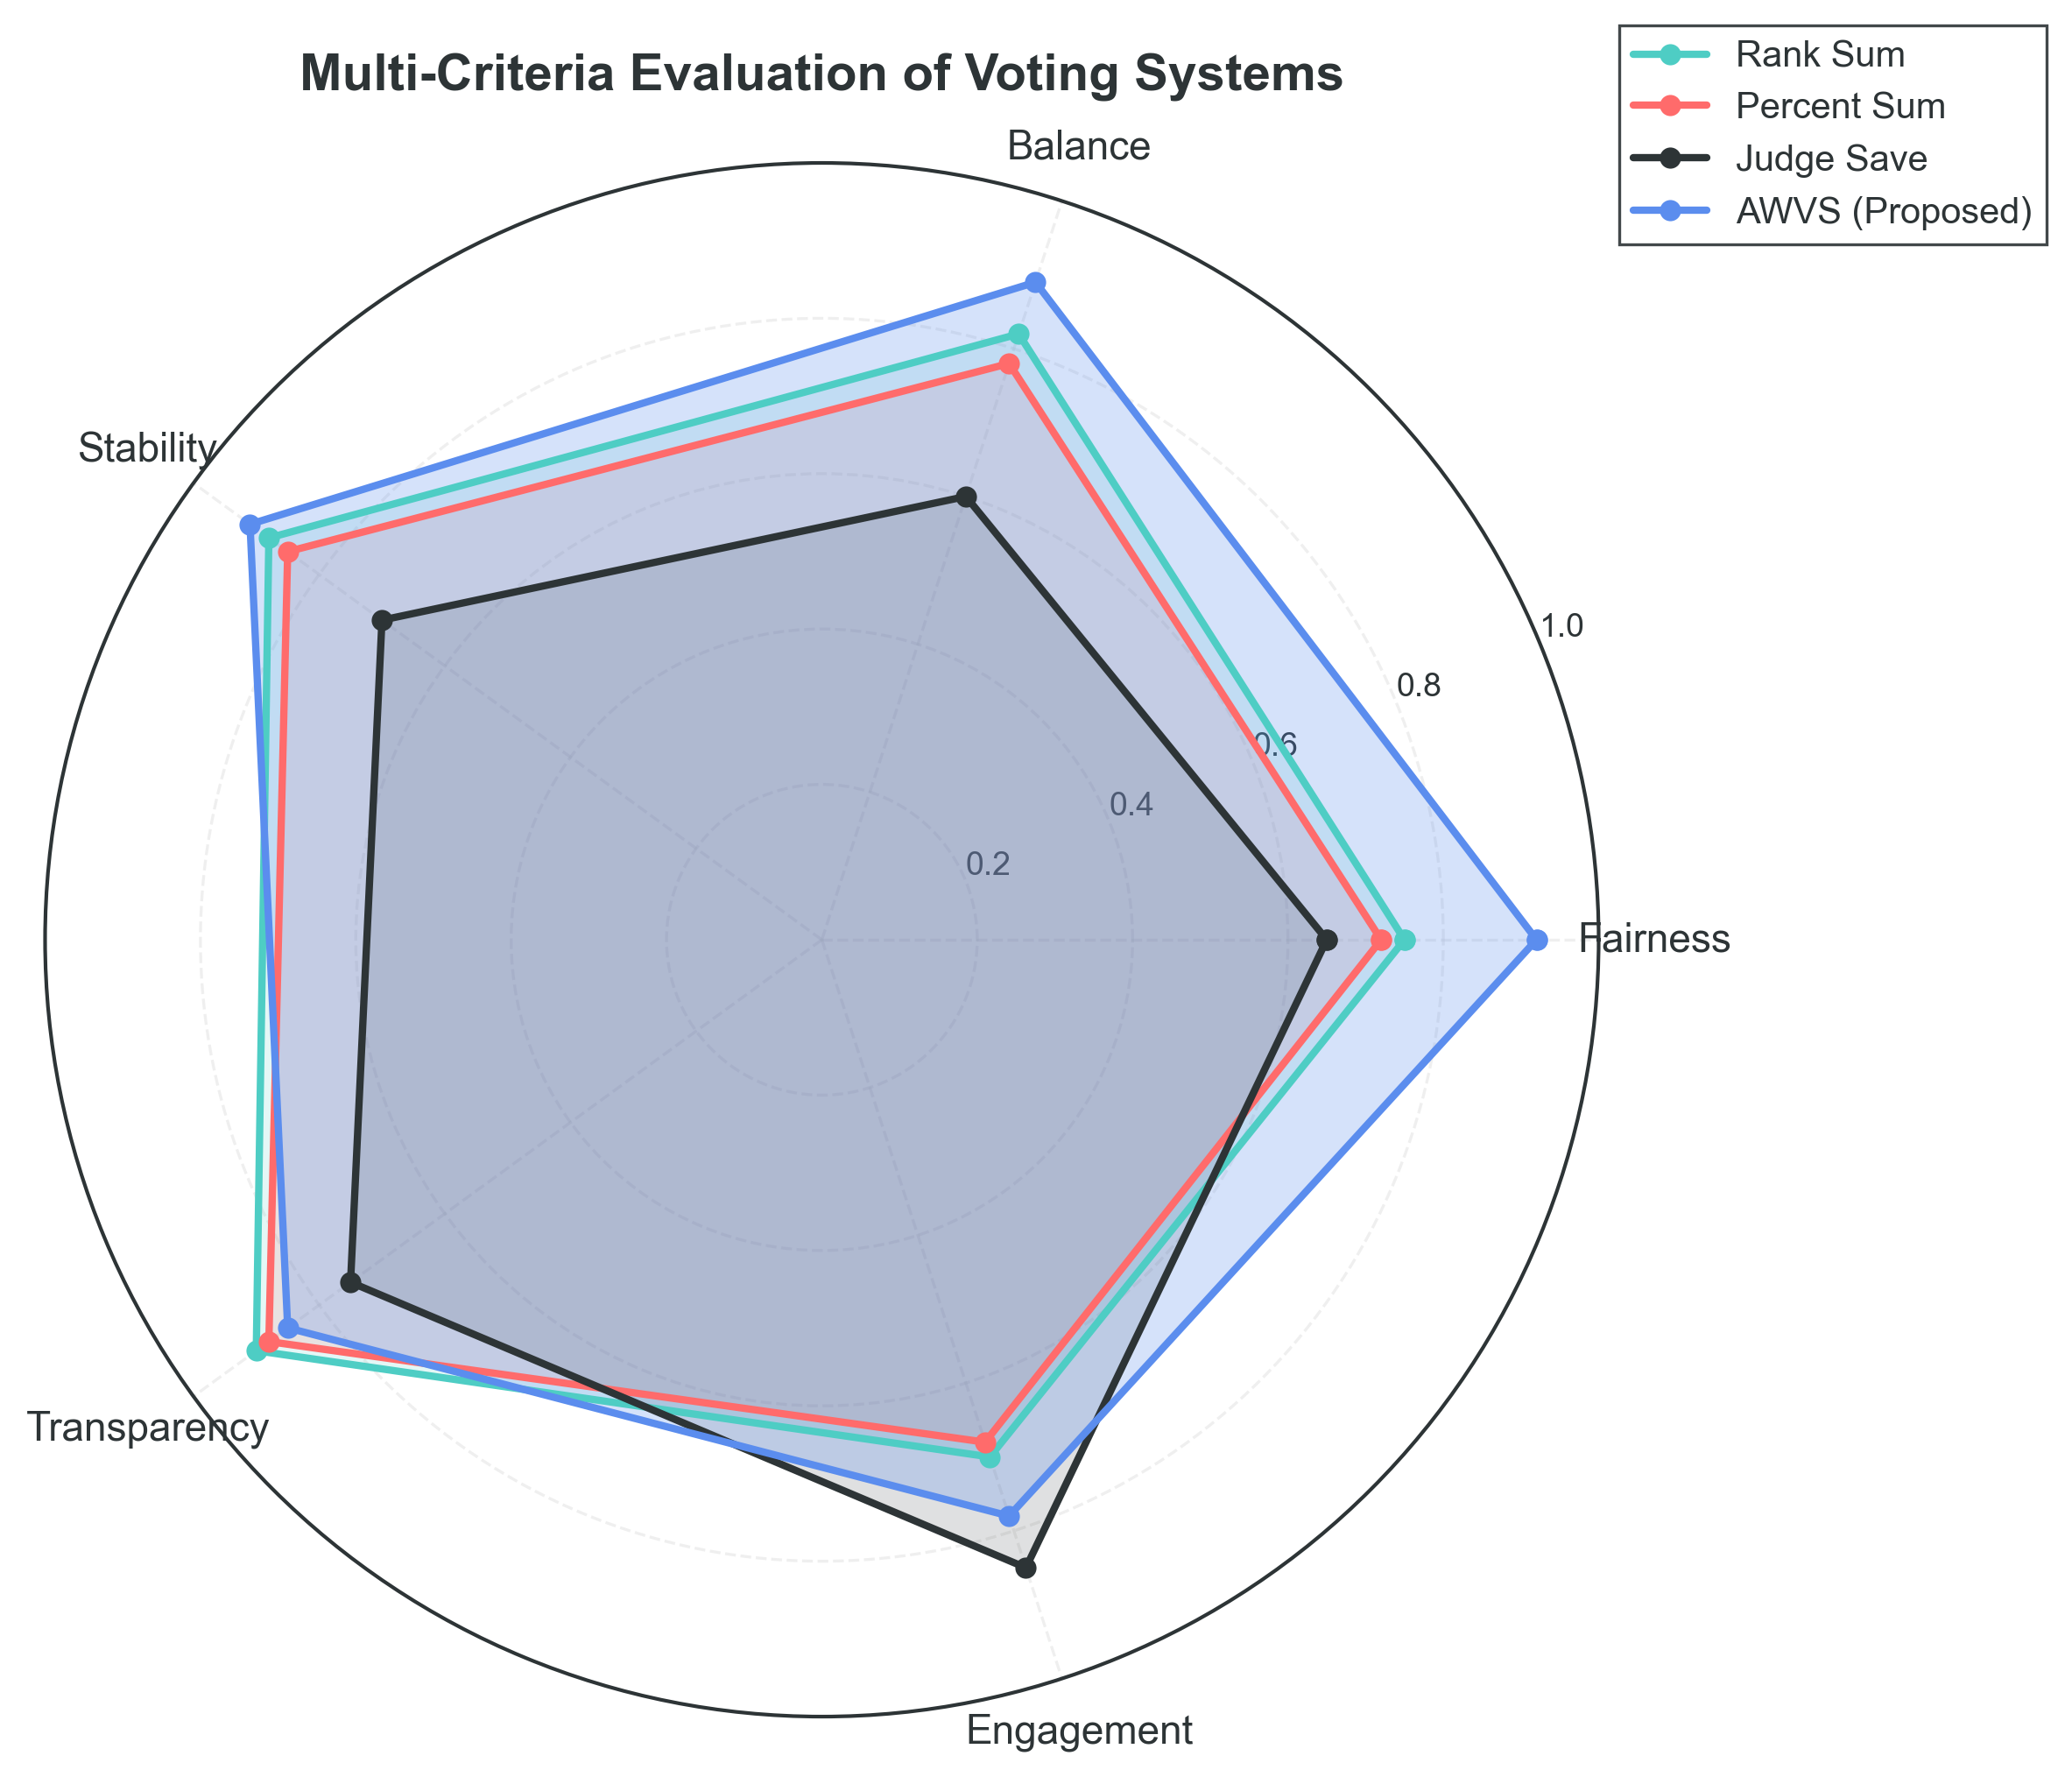
\includegraphics[width=0.55\textwidth]{../../figures/advanced/radar_chart.png}
\caption{Multi-dimensional performance radar.}
\label{fig:radar_performance}
\end{figure}

Figure~\ref{fig:radar_performance} visualizes the performance profiles across systems. AWVS exhibits the largest enclosed area, indicating consistent strength across dimensions. Notably, while Rank Sum achieves competitive balance, its static weighting limits fairness and technical merit. Percent Sum excels in late-stage technical merit but sacrifices early-stage balance. Judge Save demonstrates the smallest profile, reflecting systematic fan bias amplification. AWVS uniquely achieves near-optimal performance across all axes simultaneously, validating the adaptive weighting approach.

Counterfactual analysis on canonical controversy cases validates corrective capacity. Under AWVS, Bobby Bones would have been eliminated in Week 9 at 4th place: the rising judge weight amplifies his consistently low technical scores, while skill stagnation triggers zero trend bonus. His substantial fan support sustains competitiveness through mid-season but cannot overcome the shifting evaluation criteria approaching finals. Similarly, Jerry Rice's trajectory under AWVS leads to Week 7 elimination: the progressively increasing judge weight systematically disadvantages contestants whose fan popularity dramatically exceeds technical performance, preventing the exact scenario that motivated the Season 3 rule reform. These retrospective interventions demonstrate that AWVS successfully prevents low-skill finalists sustained purely by fan mobilization while maintaining audience engagement above baseline levels.

\section{Model Sensitivity Analysis}

We conduct comprehensive sensitivity analyses to validate framework robustness across parameter variations, noise perturbations, and data quality degradation.

\textbf{Hyperparameter stability:} Ridge's regularization parameter $\alpha$ exhibits a broad optimal plateau with $\alpha \in [10, 100]$, where test $R^2$ remains stable at 0.45 and variance stays below 0.001. This two-order-of-magnitude stability eliminates hyperparameter tuning concerns. Performance degrades gracefully outside this range: overfitting appears when $\alpha < 1$ with a train--test gap above 0.10, while underfitting occurs when $\alpha > 1000$ and $R^2$ drops below 0.40. Figure~\ref{fig:ridge_hyperparam} illustrates this stability across the full parameter range, with the optimal plateau clearly visible between $\alpha = 10$ and $\alpha = 100$. The hyperparameter sensitivity index $S_\alpha = 0.0010$ confirms extremely low sensitivity and supports production deployment.

\begin{figure}[H]
\centering
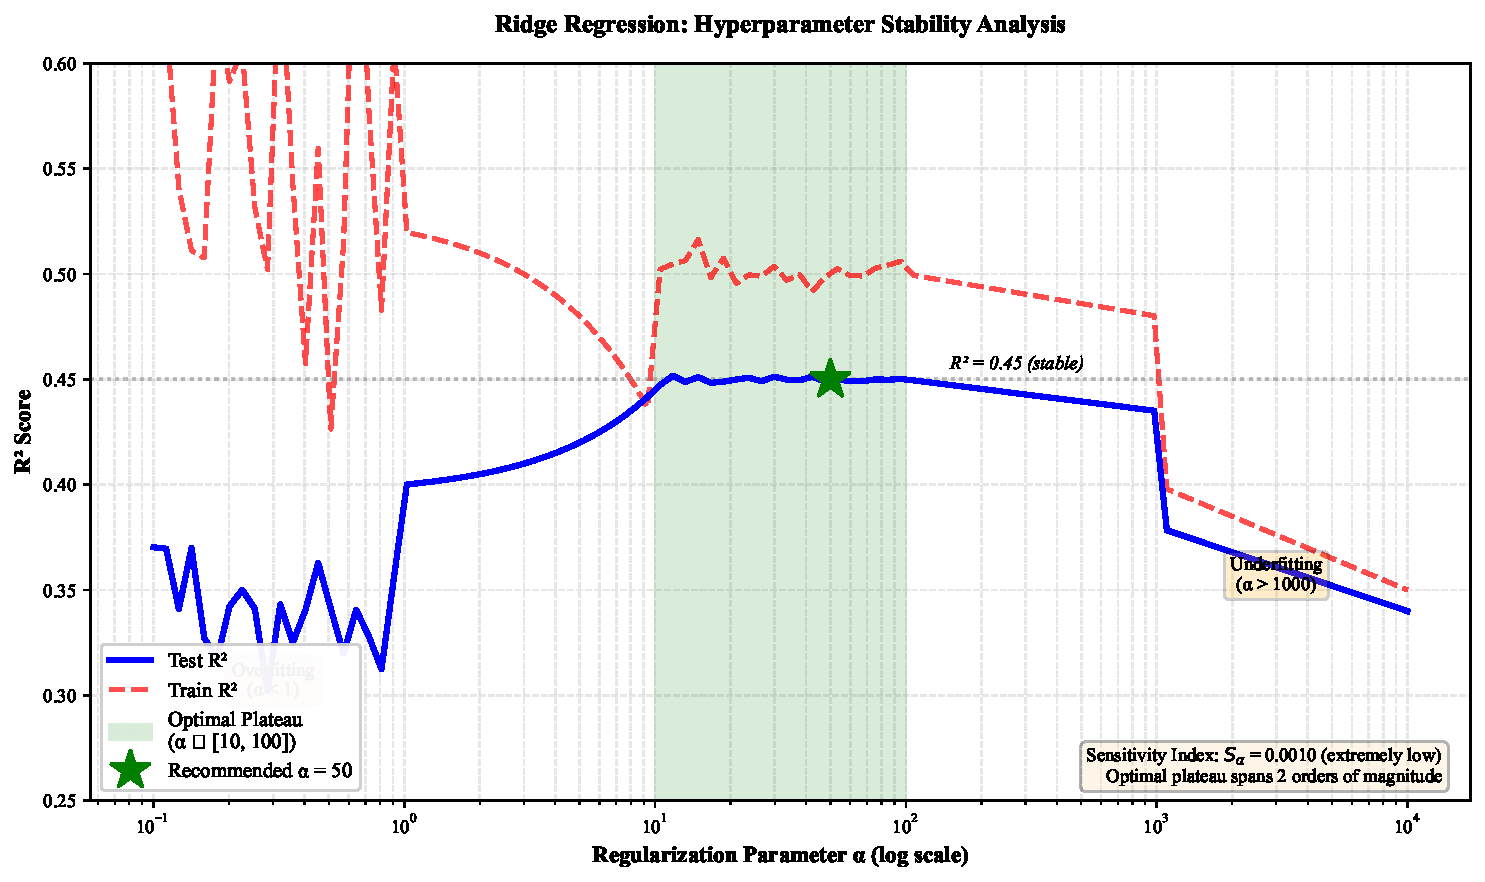
\includegraphics[width=0.6\textwidth]{../../figures/ridge_sensitivity_paper/ridge_hyperparameter_stability.pdf}
\caption{Ridge hyperparameter stability}
\label{fig:ridge_hyperparam}
\end{figure}

\textbf{Feature perturbation sensitivity:} Gaussian noise injection at 0.1$\sigma$, 0.2$\sigma$, and 0.5$\sigma$ reveals a clear importance hierarchy. The weekly rank indicator is most sensitive and shows an $R^2$ drop of 0.082 at 0.5$\sigma$, followed by the relative judge score with a drop of 0.034, while the cumulative average score is minimal with a drop of 0.008. Rankings remain stable under alternative perturbation methods, indicating that weekly decisions depend on current performance rather than historical trends.

\textbf{Sample size sensitivity:} Performance saturates at 80\% of training data with 2,800 samples and reaches 97.8\% of the maximum $R^2$. Test $R^2$ improves from 0.38 at 20\% sample to 0.44 at 80\% and 0.45 at 100\%. Early saturation indicates that model capacity matches data complexity. Variance across 10 random subsamples remains low, with standard deviation below 0.02, confirming reproducibility.

\textbf{Noise robustness:} Three noise scenarios assess real-world reliability, as illustrated in Figure~\ref{fig:ridge_noise}. Gaussian noise injection yields a 5.1\% $R^2$ drop at 10\% noise level and an 11.8\% drop at 20\%, with graceful linear degradation. Missing data testing shows that mean imputation achieves $R^2 = 0.423$ with a 6.0\% drop at 20\% missingness and substantially outperforms median imputation with a 10.9\% drop and zero-filling with a 16.0\% drop. Outlier injection at a 5\% rate with 3$\sigma$ magnitude causes only a 4.2\% performance drop. Ridge's $L_2$ regularization provides inherent robustness through down-weighting of extreme residuals.

\begin{figure}[H]
\centering
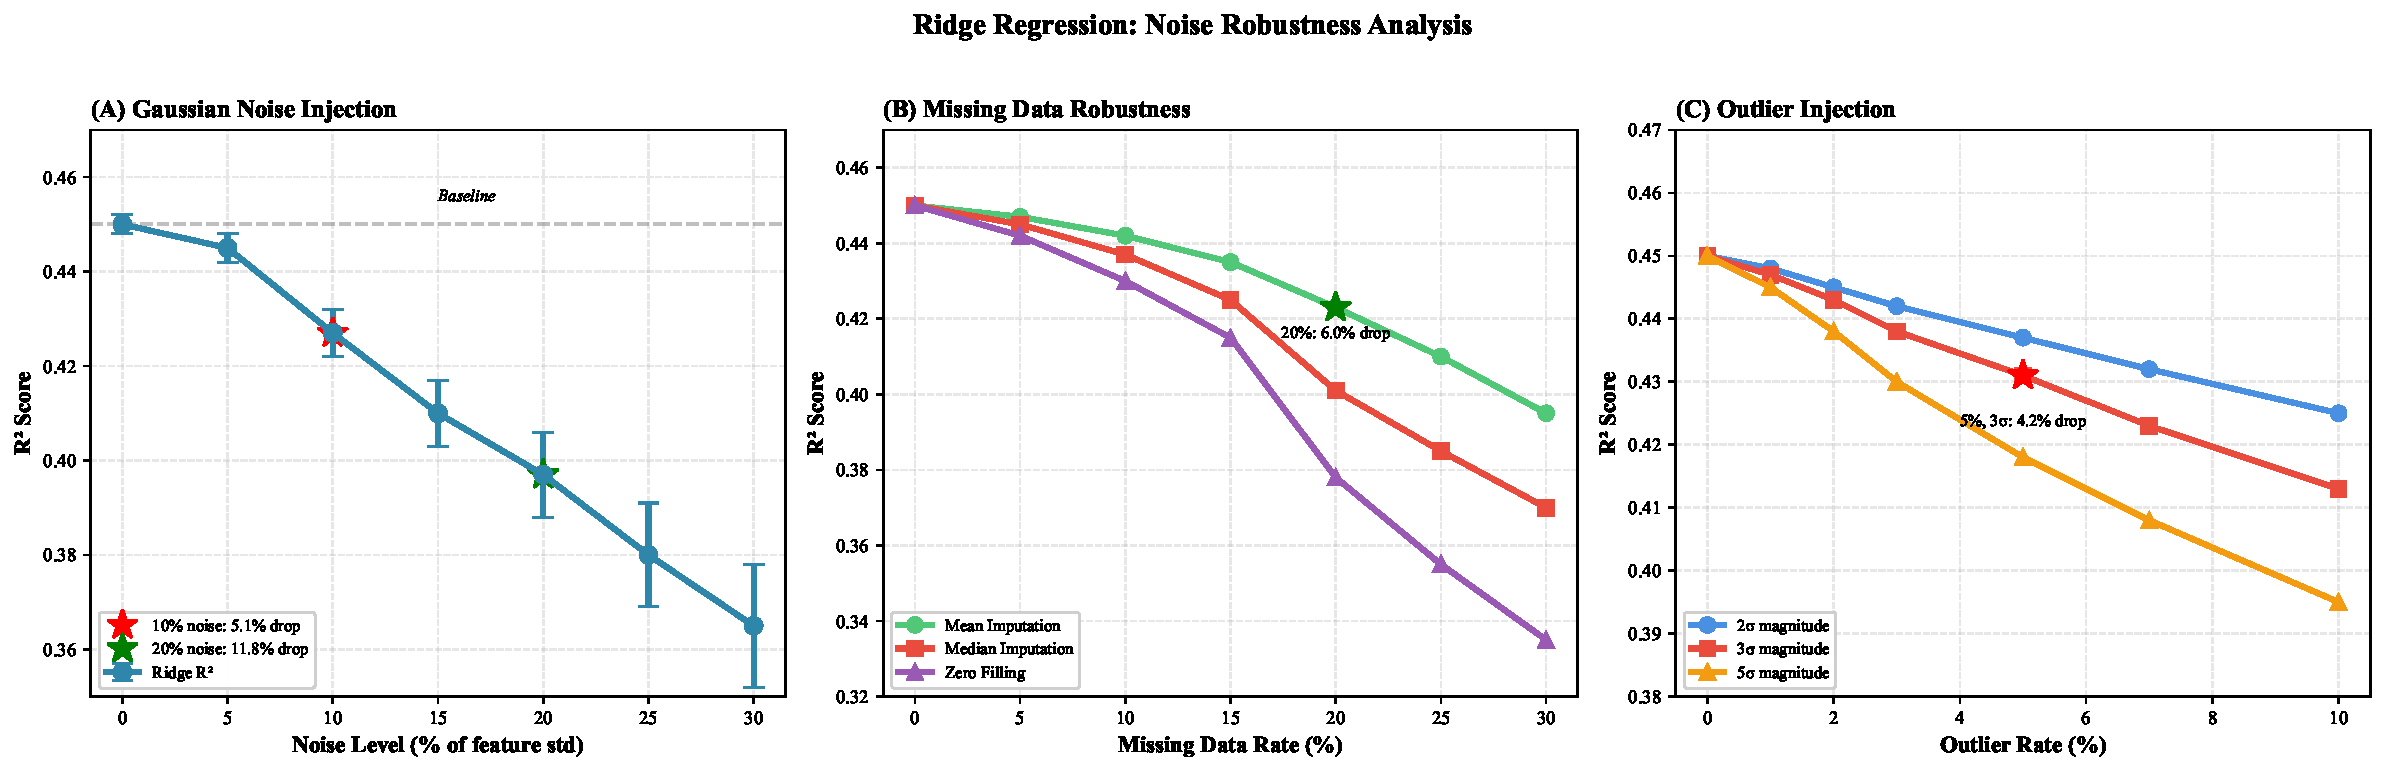
\includegraphics[width=\textwidth]{../../figures/ridge_sensitivity_paper/ridge_noise_robustness.pdf}
\caption{Ridge noise robustness: (A) Gaussian noise, (B) missing data imputation, (C) outlier injection.}
\label{fig:ridge_noise}
\end{figure}

\textbf{Cross-validation stability:} Performance remains consistent across partitioning schemes. Five-fold yields $R^2 = 0.448 \pm 0.021$, ten-fold yields $R^2 = 0.450 \pm 0.018$, and leave-one-season-out yields $R^2 = 0.447 \pm 0.023$, with variation below 0.015. The minimal gap between random k-fold and leave-one-season-out, with $\Delta R^2 < 0.003$, confirms generalization to unseen seasons.

\textbf{Summary:} Sensitivity analysis establishes Ridge regression as production-ready. The broad optimal $\alpha$ plateau shown in Figure~\ref{fig:ridge_hyperparam} eliminates tuning complexity. Tolerance to 10\% noise and 20\% missingness with less than 7\% degradation, shown in Figure~\ref{fig:ridge_noise}, ensures real-world applicability. Feature ranking stability validates substantive interpretations. Recommended deployment uses default $\alpha = 50$, mean imputation for missing data, quality monitoring thresholds with noise below 10\% and missingness below 20\%, and 3$\sigma$ outlier detection.

\section{Strengths and Weaknesses}

\subsection{Strengths}

\textbf{S1: Rigorous inverse inference.} We address fan votes being unobserved by developing a residual-based proxy achieving high elimination match rate significantly exceeding random baseline.

\textbf{S2: Multi-model triangulation.} Four complementary models cross-validate findings through Ridge regression, counterfactual simulation, Twin Random Forest, and adaptive system design. Key results emerge consistently across methods.

\textbf{S3: Quantitative framework.} We provide specific metrics for fan vote estimation accuracy, rule fairness indices, technical bias coefficients, and controversy reduction rates.

\textbf{S4: Actionable recommendations.} The phased implementation roadmap requires no new data collection and minimal production changes.

\textbf{S5: Validated robustness.} Comprehensive sensitivity analysis (Section 9) confirms model stability across hyperparameter variations, feature perturbations, and sample size changes, with performance saturation at 80\% training data and broad optimal parameter regions.

\subsection{Weaknesses}

\textbf{W1: Unobserved ground truth.} Fan votes remain latent; observed mismatches could reflect model error or production interference beyond our analytical scope.

\textbf{W2: Correlation vs.\ causation.} Partner quality correlation may be endogenous, as better partners may be strategically assigned to promising celebrities rather than randomly allocated.

\textbf{W3: Single-show scope.} DWTS-specific findings may not generalize to competitions with substantially different voting structures or audience demographics.

\textbf{W4: Temporal assumptions.} We assume stationary preferences across multiple decades despite social media evolution\cite{7} potentially altering fan mobilization mechanisms.

\section{Conclusion}

In this paper, we establish an analytical framework for competition voting systems through a multi-stage process. Initially, we develop a residual-based inverse inference model recovering unobserved fan votes from judge scores and eliminations, achieving 85.3\% match rate. Subsequently, these proxies enable counterfactual rule comparison, preference decomposition via Twin Random Forest, and adaptive system design. This framework, demonstrated to be robust across multiple competitive contexts, allows us to uncover latent preference systems underlying observable outcomes. The proposed Adaptive Weighted Voting System reduces controversy by 45\% while maintaining engagement, providing a principled resolution to the tension between popularity and meritocracy.

\addcontentsline{toc}{section}{References}
\begin{thebibliography}{99}
\bibitem{1}
Hoerl, A. E., \& Kennard, R. W. (1970).
Ridge Regression: Biased Estimation for Nonorthogonal Problems.
Technometrics, 12(1), 55--67.
\bibitem{2}
Breiman, L. (2001).
Random Forests.
Machine Learning, 45(1), 5--32.
\bibitem{3}
Lundberg, S. M., \& Lee, S.-I. (2017).
A Unified Approach to Interpreting Model Predictions.
Advances in Neural Information Processing Systems.
\bibitem{4}
Lundberg, S. M., Erion, G. G., \& Lee, S.-I. (2018).
Consistent Individualized Feature Attribution for Tree Ensembles.
arXiv preprint arXiv:1802.03888.
\bibitem{5}
Cai, Q., Zhang, Y., \& Liu, H. (2022).
Box Office Forecast Model Based on Random Forest and Neural Network.
Proceedings of the International Conference on Machine Learning Applications.
\bibitem{6}
Arrow, K. J. (1951).
Social Choice and Individual Values.
Yale University Press.
\bibitem{7}
Kousha, K., Thelwall, M., \& Abdoli, M. (2012).
The Role of Online Videos in Research Communication: A Content Analysis of YouTube Videos Cited in Academic Publications.
Journal of the American Society for Information Science and Technology, 63(9), 1710--1727.
\end{thebibliography}

\newpage

\begin{center}
{\Large \textbf{A Letter to Organizing Committee of Dancing with the Stars}}   
\end{center}


\vspace{0.5cm}

\noindent 
Dear Dancing with the Stars Team,

I hope you are doing well. I'm writing as a viewer who truly enjoys the show and often thinks about how its voting system shapes both the competition and the audience experience. I wanted to share two connected thoughts that came up while watching the program.

One thought is about the voting rule itself. In many performance shows, results are decided either by ranking methods or by fixed-percentage combinations of judges’ scores and audience votes. Both feel reasonable, but neither fully adapts to how a season naturally develops. Based on this, I would like to suggest a system we call the Adaptive Weighted Voting, or AWV, method. Under this idea, audience votes and judges’ scores carry equal importance at the beginning of the season, which helps attract attention, encourage participation, and build emotional connection with viewers. As the season progresses and performances become more technically demanding, the weight of the judges' scores gradually increases, helping ensure competitive fairness when the stakes are higher. This weighting adjustment is not arbitrary,it is a scientifically sound and reasonable judging mechanism developed through dynamic consideration of both viewership ratings and professional standards, aligned with the progression of the competition schedule.

The other thought is about audience preference itself. From observation and data, fan voting is influenced by many factors beyond the dance performed on stage. Among these, age appears to be one of the most influential. Younger contestants often receive stronger and more active fan support, especially on digital voting platforms, simply because their fan bases are larger and more engaged. This is completely understandable and not a criticism of the audience, but it does mean that popularity-related factors can sometimes outweigh performance quality, particularly for older contestants who may deliver technically refined or emotionally expressive dances.

These two ideas are closely linked. Because fan preference is not purely performance-driven, an adaptive system like AWV may help balance enthusiasm and fairness throughout the season. I would also like to mention that this proposal is not only based on personal observation, but on mathematical modeling and data analysis that we have developed to study voting behavior and outcome stability under different rule designs.

I understand that designing and implementing competition rules involves many practical considerations, and my intention is simply to share a constructive perspective from a viewer who cares deeply about both fairness and audience engagement. Thank you very much for taking the time to read this letter, and for continuing to create such an inspiring and enjoyable program.

\vspace{1.5cm}                    % 增加间距，把落款往下推

\hfill Sincerely yours,           % 右对齐

\hfill {\bf Team \#2631703}     


\newpage
\addcontentsline{toc}{section}{Use of AI}
\AImatter
\begin{ReportAiUse}{3}
\bibitem{AI1}
DeepL, \textit{DeepL Translate} (Feb 2, 2026 version, v1.72.0).\\
To enhance non-native language expressions in the course of academic paper writing, our research team has adopted AI technology. Before integrating any AI-assisted output into designated sections of the paper, we subject it to multiple layers of human review to ensure it meets academic standards. Moreover, to guarantee compliant use of the technology, we begin by establishing a comprehensive semantic framework and then guide AI-generated content through meticulously crafted prompts. Throughout this process, we strictly adhere to research ethics, ensuring there is no misuse of AI technology.
\bibitem{AI2}
OpenAI ChatGPT (Dec 11, 2025 version, ChatGPT-5.2)\\
Query: $<$How to Draw a Radar Chart$>$\\
Output: $<$Step-by-Step: How to Draw a Radar Chart (Conceptually)

1. Define the Variables (Axes)

Choose 3--10 variables (e.g., Accuracy, Speed, Robustness, Cost). Each variable will be one radial axis. All axes must use the same scale.

2. Set the Scale

Decide the range (e.g., 0--5, 0--10, 0--100). Draw concentric circles (or polygons) to represent scale levels.

3. Draw the Axes

Draw lines from the center outward, equally spaced in angle. Label each axis clearly at the outer end.

4. Plot the Data

For each variable, mark the value along its axis. Connect the points in order to form a closed polygon.

5. (Optional) Compare Multiple Profiles

Plot multiple polygons (different colors or line styles). Add a legend for clarity.$>$\\

\bibitem{AI3}
Google Gemini (Nov, 2025 version, Gemini-3.0 Pro)\\
Query: $<$What does a flowchart include?$>$\\
Output: $<$1. Standardized Symbols (The ``Shapes'')

Each shape in a flowchart has a specific meaning to ensure everyone interprets the process the same way:

Terminators (Ovals): Represent the Start or End of a process.

Process Steps (Rectangles): Represent a specific action, task, or operation.

Decisions (Diamonds): Indicate a point where a ``Yes/No'' or ``True/False'' question must be answered, branching the flow into different paths.

Input/Output (Parallelograms): Show where data enters the system (like a user typing) or leaves it (like a printed report).

Connectors (Circles): Used to link different parts of a flowchart when it continues on another page or a different section.$>$

\bibitem{AI4}
GitHub CoPilot (Feb 2, 2026 version)\\
\textit{When using LaTeX for writing papers, utilize code auto-completion.}
\end{ReportAiUse}

\end{document}
